%---------------------------------------------------------------------------%
%-                                                                         -%
%-                           LaTeX Template                                -%
%-                                                                         -%
%---------------------------------------------------------------------------%
%- Copyright (C) Huangrui Mo <huangrui.mo@gmail.com>
%- This is free software: you can redistribute it and/or modify it
%- under the terms of the GNU General Public License as published by
%- the Free Software Foundation, either version 3 of the License, or
%- (at your option) any later version.
%---------------------------------------------------------------------------%
%->> Document class declaration
%---------------------------------------------------------------------------%
\documentclass[doublesided]{Style/ucasthesis}%
%- Multiple optional arguments:
%- [<singlesided|doublesided|printcopy>]% set one or two sided eprint or print
%- [showmj]% show confidential information
%- [draftversion]% show draft version information
%- [fontset=<adobe|...>]% specify font set to replace automatic detection
%- [scheme=plain]% thesis writing of international students
%- [standard options for ctex book class: draft|paper size|font size|...]%
%---------------------------------------------------------------------------%
%->> Document settings
%---------------------------------------------------------------------------%
\usepackage[super,myhdr]{Style/artratex}% document settings
%- usage: \usepackage[option1,option2,...,optionN]{artratex}
%- Multiple optional arguments:
%- [bibtex|biber]% set bibliography processor and package
%- [<numbers|super|authoryear|alpha>]% set citation and reference style
%- <numbers>: textual: Jones [1]; parenthetical: [1]
%- <super>: textual: Jones superscript [1]; parenthetical: superscript [1]
%- <authoryear>: textual: Jones (1995); parenthetical: (Jones, 1995)
%- <alpha>: textual: not available; parenthetical: [Jon95]
%- [geometry]% reconfigure page layout via geometry package
%- [lscape]% provide landscape layout environment
%- [myhdr]% enable header and footer via fancyhdr package
%- [color]% provide color support via xcolor package
%- [background]% enable page background
%- [tikz]% provide complex diagrams via tikz package
%- [table]% provide complex tables via ctable package
%- [list]% provide enhanced list environments for algorithm and coding
%- [math]% enable some extra math packages
\usepackage{Style/artracom}% user defined commands
\usepackage{amsmath}
\usepackage[siunitx]{circuitikz}
\usepackage{float}
% ---------------------------------------------------------------------------%
%->> Document inclusion
%---------------------------------------------------------------------------%
%\includeonly{Tex/Chap_1,...,Tex/Chap_N}% selected files compilation
%---------------------------------------------------------------------------%
%->> Document content
%---------------------------------------------------------------------------%
\begin{document}
%-
%-> Frontmatter: title page, abstract, content list, symbol list, preface
%-
\frontmatter% initialize the environment

\title{硬件电路设计笔记}
\author{李涛 \\
% Institution1 address\\
{\tt\small litroncn@gmail.com}
% For a paper whose authors are all at the same institution,
% omit the following lines up until the closing ``}''.
% Additional authors and addresses can be added with ``\and'',
% just like the second author.
% To save space, use either the email address or home page, not both
}
\chinesedate{2018~年~1~月}
\maketitle
% title page, abstract, dedication
% \intotoc{\contentsname}% add link to contents table and bookmark
\tableofcontents% contents catalog
% \intotoc{\listfigurename}% add link to contents table and bookmark
% \listoffigures% figures catalog
% \intotoc{\listtablename}% add link to contents table and bookmark
% \listoftables% tables catalog
% \chapter{符号列表}

\section*{字符}
\nomenclatureitem[\textbf{Unit}]{\textbf{Symbol}}{\textbf{Description}}
\nomenclatureitem[$\Unit{m^{2} \cdot s^{-2} \cdot K^{-1}}$]{$R$}{the gas constant}
\nomenclatureitem[$\Unit{m^{2} \cdot s^{-2} \cdot K^{-1}}$]{$C_v$}{specific heat capacity at constant volume}
\nomenclatureitem[$\Unit{m^{2} \cdot s^{-2} \cdot K^{-1}}$]{$C_p$}{specific heat capacity at constant pressure}
\nomenclatureitem[$\Unit{m^{2} \cdot s^{-2}}$]{$E$}{specific total energy}
\nomenclatureitem[$\Unit{m^{2} \cdot s^{-2}}$]{$e$}{specific internal energy}
\nomenclatureitem[$\Unit{m^{2} \cdot s^{-2}}$]{$h_T$}{specific total enthalpy}
\nomenclatureitem[$\Unit{m^{2} \cdot s^{-2}}$]{$h$}{specific enthalpy}
\nomenclatureitem[$\Unit{kg \cdot m \cdot s^{-3} \cdot K^{-1}}$]{$k$}{thermal conductivity}
\nomenclatureitem[$\Unit{kg \cdot m^{-1} \cdot s^{-2}}$]{$S_{ij}$}{deviatoric stress tensor}
\nomenclatureitem[$\Unit{kg \cdot m^{-1} \cdot s^{-2}}$]{$\tau_{ij}$}{viscous stress tensor}
\nomenclatureitem[$\Unit{1}$]{$\delta_{ij}$}{Kronecker tensor}
\nomenclatureitem[$\Unit{1}$]{$I_{ij}$}{identity tensor}

\section*{算子}
\nomenclatureitem{\textbf{Symbol}}{\textbf{Description}}
\nomenclatureitem{$\Delta$}{difference}
\nomenclatureitem{$\nabla$}{gradient operator}
\nomenclatureitem{$\delta^{\pm}$}{upwind-biased interpolation scheme}

\section*{缩写}
\nomenclatureitem{CFD}{Computational Fluid Dynamics}
\nomenclatureitem{CFL}{Courant-Friedrichs-Lewy}
\nomenclatureitem{EOS}{Equation of State}
\nomenclatureitem{JWL}{Jones-Wilkins-Lee}
\nomenclatureitem{WENO}{Weighted Essentially Non-oscillatory}
\nomenclatureitem{ZND}{Zel'dovich-von Neumann-Doering}

% list of symbols, preface content
%-
%-> Mainmatter
%-
\mainmatter% initialize the environment
%---------------------------------------------------------------------------%
%->> Main content
%---------------------------------------------------------------------------%

\chapter{发光二极管}
\label{chap:introduction}

发光二极管也是由一个PN结构成,具有单向导电性。但其正向工作电压(开启电压)比普通二极管高,约为1~2.5V,反向击穿电压比普通二极管低,约5V左右。当正向电流达到1mA左右时开始发光,发光强度近似与工作电流成正比;但工作电流达到一定数值时,发光强度逐渐趋于饱和,与工作电流成非线性关系。一般小型发光二极管正向工作电流为10~20mA,最大正向工作电流为30~50mA。

发光二极管的外形可以做成矩形、圆形、字形、符号形等多种形状,又有红、绿、黄、橙、红外等多种颜色。它具有体积小、功耗低、容易驱动、光效高、发光均匀稳定、响应速度快以及寿命长等特点。

\begin{figure}[!htbp]
    \centering
    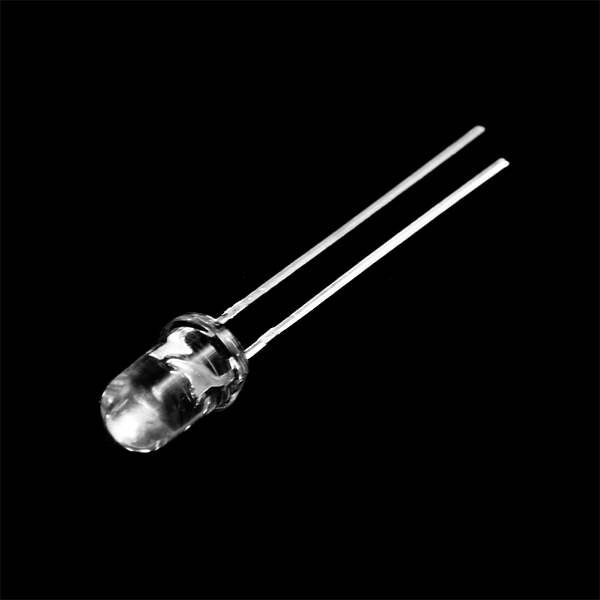
\includegraphics[width=0.45\textwidth]{08285-01}
    \caption{LED - Super Bright Green}
    \label{fig:08285-01}
\end{figure}

\section{典型电路}
LED电路是由电源,电阻,发光二极管串联组成的, 如图~\ref{fig:led_circuit}

\begin{figure}[H]
    \centering
    % 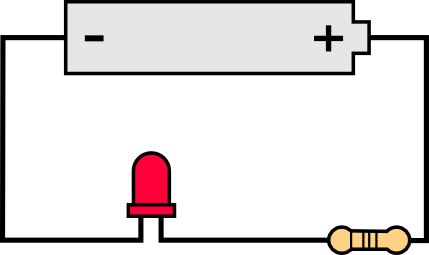
\includegraphics[width=0.8\textwidth]{led_circuit}
    \begin{circuitikz}
      \draw[color=black, thick, scale=2]
      (0,0)
      to[R=$R_1$] (2,0)
      to[empty led](4,0)
      to[short] (4,0) -- (4,2)
      to[battery1] (0,2)
      to[short] (0,2) -- (0,0)
      ;
    \end{circuitikz}
    \caption{LED Circuit}
    \label{fig:led_circuit}
\end{figure}


\section{电阻计算}

下图来自深圳市昱申科技有限公司的LED模块\href{https://www.sparkfun.com/datasheets/Components/YSL-R542G5C-A14.pdf}{YSL-R542G5C-A14}

\begin{figure}[H]
    \centering
    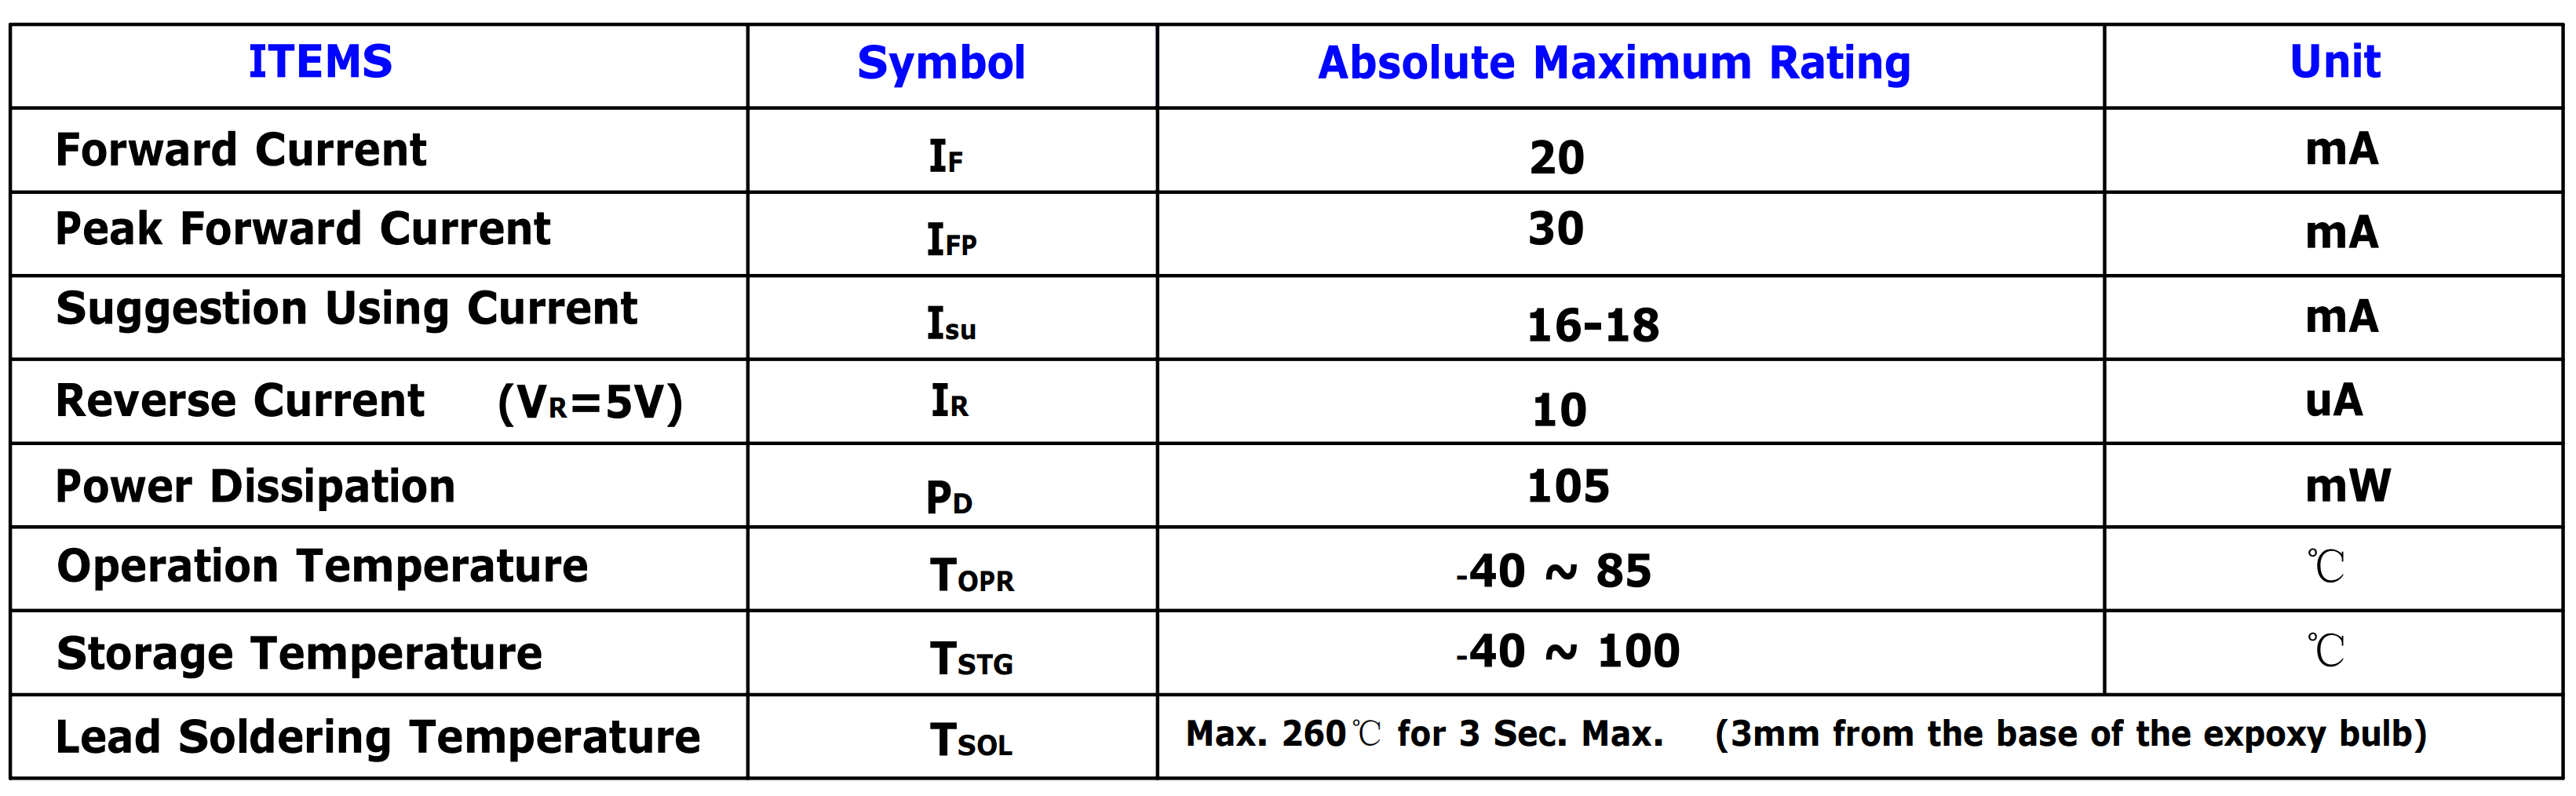
\includegraphics[width=0.8\textwidth]{led_current}
    \caption{LED Current}
    \label{fig:led_current}
\end{figure}

\begin{figure}[H]
    \centering
    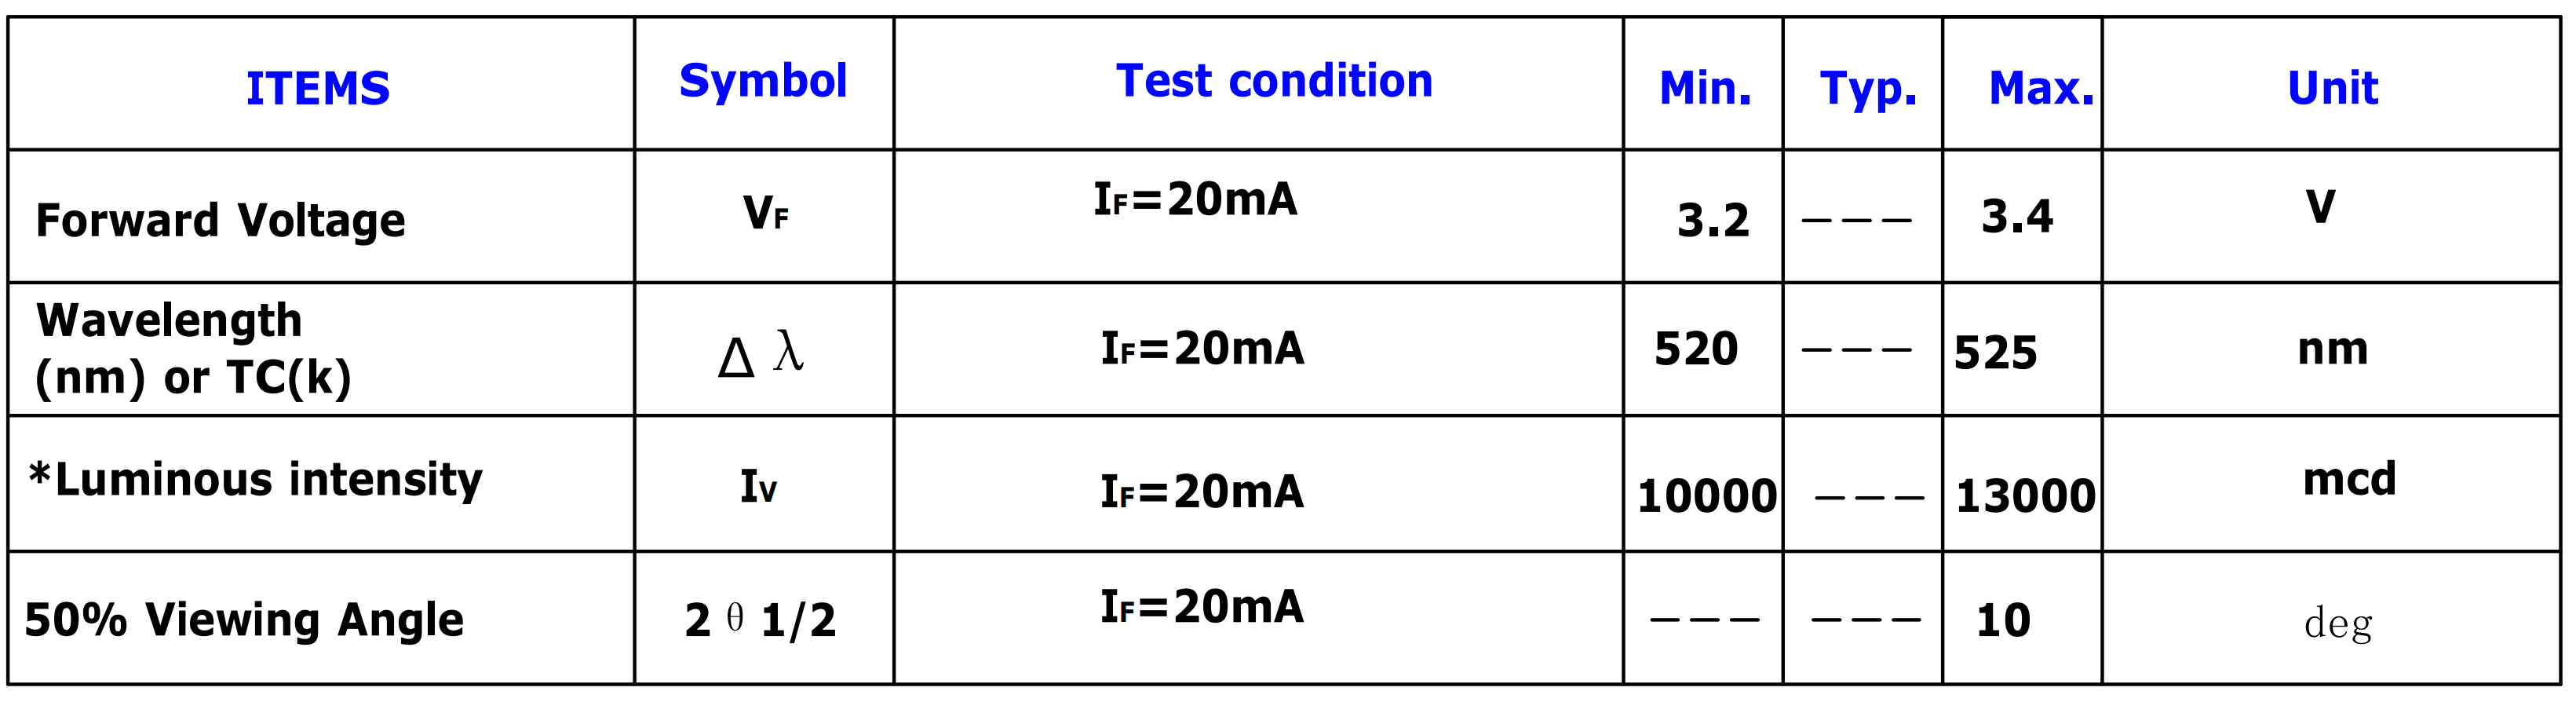
\includegraphics[width=0.8\textwidth]{led_voltage}
    \caption{LED Voltage}
    \label{fig:led_voltage}
\end{figure}

需要注意的是这几项Forward Current, Peak Forward Current, Suggestion Using Current和Forward Voltage,建议使用电流是$I_{su}$, $16mA \leq I_{su} \leq 18mA$, Forward Voltage $V_f \approx 3.3V$, $V_{cc}$应大于$V_f$ 这里选择$I_{su}=17mA, V_{cc}=5V$, 功耗$P=U*I_{su}$, 尽量使功耗最低。

\begin{equation}\label{eq:led_calc_r}
\begin{aligned}
        V_{cc} & = V_R + V_f \\
        R & = \frac{V_{cc} - V_f}{I_{su}} \\
        R & = \frac{5V - 3.3V}{17mA} \\
        R & = 100\Omega \\
        P & = V_{cc} * I_{su} \\
        P & = 5V * 17mA = 85mW
\end{aligned}
\end{equation}

LED说明 \\
\indent $\blacksquare$ LED导通才发光 \\
\indent $\blacksquare$ LED通过电流太大容易损坏(典型最大值20毫安) \\
\indent $\blacksquare$ LED反向电压过大容易损坏 \\


\begin{figure}[H]
    \centering
    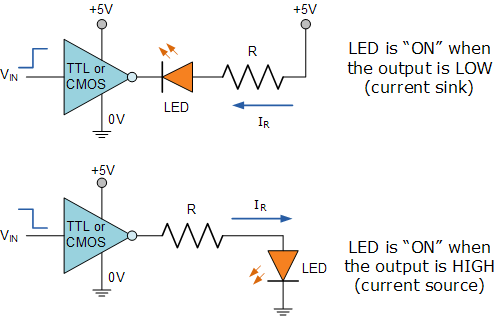
\includegraphics[width=0.8\textwidth]{ic_driver_circuit}
    \caption{IC Driver Circuit}
    \label{fig:ic_driver_circuit}
\end{figure}

\begin{figure}[H]
    \centering
    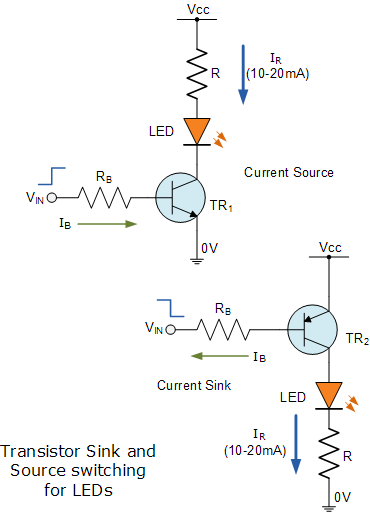
\includegraphics[width=0.8\textwidth]{transistor_driver_circuit}
    \caption{Transistor Driver Circuit}
    \label{fig:transistor_driver_circuit}
\end{figure}

\textbf{为什么电路要串联电阻?}

\textbf{为什么要选择$V_{cc}=5V$?}

\textbf{串联电阻的作用是什么?}


\chapter{放大电路}
\label{chap:amplifier}

% \begin{tikzpicture}[scale=2]
\begin{circuitikz}[american,line width=1pt]
  \draw
    (0,0) to [short,o-] (6,0){} % Baseline for connection to ground
    % Input and ground
    (0,1) node[]{\large{\textbf{$v_i$}}}
    % Connection of passive components
    (5,0) node[ground]{} node[circ](4.5,0){}
    (0,2) to [C, l_=$C_1~10\mu$, o-] (1.5,2)
    % to [R,l_=$R_1$,](1.5,2)
    (1.5,2) to node[short]{}(3,2)
    % (1.5,2) to [C, l=$C_2$, *-] (1.5,3) -| (5,3)
    % (2.2,2) to [R, l=$R_2$, *-*] (2.2,3)
    (2.2,2) to node[short]{}(2.2,3)
    (2.2,3) to [R, l=$R_1$100k, -*] (2.2,5) -| (3,5)
    % Transistor Bipolar Q1
    (3,0) to [R,l=$R_{\rm E}$2k,*-] (3,1.5)
    to [Tnpn,n=npn1] (3,2.5)
    (npn1.E) node[right=3mm, above=5mm]{$Q_1$} % Labelling the NPN transistor
    % (4,0) to [pC, l_=$C_4$, *-] (4, 1.5)--(3,1.5)
    (2.2,0) to [R, l=$R_2$22k, *-] (2.2,1.5)
    (2.2,1.5) to node[short]{}(2.2,2)

    (3,2.5) to node[short]{}(3,3)
    (3,5) to [R, n=pot1, l_=$R_4$, *-] (3,3)
    % (3,5) to [R, l=$R_6$, *-] (5,5)
    (0,5) to [short, -] (6,5)
    (4,5) to [C, l_=$C_30.1\mu$, *-] (4,4) node[ground]{}
    (5,5) to [C, l_=$C_410\mu$, *-] (5,4) node[ground]{}

    (0,5) to [battery,l_=$15V$] (0,4) node[ground]{}
    % to [short,*-o](5,5.5) node[right]{$V_{\rm cc}=15 V$}
    % Mosfet Transistors
    % (5,3) to [Tnigfetd,n=mos1] (5,5)
    % (mos1.B) node[anchor=west]{$Q_2$} % Labelling MOSFET Q2 Transistor
    % (pot1.wiper)  to [R, l=$R_7$] (4.5,4) -| (mos1.G)
    % (5,1.5) to [Tpigfetd,n=mos2] (5,2.5)
    % (5,0) to (mos2.S)
    % (3,2.5) to [R, l=$R_8$, *-] (4.5,2.5)
    % -| (mos2.G)
    % (mos2.B) node[anchor=west]{$Q_3$} % Labelling MOSFET Q3 Transistor
    % Output
    (6,3) to [C, l=$C_2$,-*](3,3)
    % (5,3) to [short,-*] (3,3){}
    (6,3) to [short,-o] (6,2){}
    % (mos1.S)--(mos2.D)
    (6,0) to [short,-o] (6,1){} node[above=7mm]{\large{\textbf{$v_o$}}}
    ;
% \end{tikzpicture}
\end{circuitikz}

\begin{figure}[htbp]
\begin{center}
\begin{circuitikz}[american,line width=1pt]
\draw (0,0) node[pnp](pnp){$Q_2$};
\draw ++(0,2) node[npn](npn){$Q_1$};
\draw (-4,1) node[op amp,yscale=1](opamp){} ;
\draw (npn.C) to[short,-o] ++(0,0.5) node[right]{$V_{\rm CC}$};
\draw (pnp.C) to[short,-o] ++(0,-0.5) node[right]{$V_{\rm EE}$};
\path (pnp.E) -- coordinate[midway](X) ( npn.E);
\draw (pnp.E) to[short,-*] (X) to[short] (npn.E);
\draw (X) to[short] ++(1.5,0) coordinate(A) to[short,-o] ++(0.5,0) node[right]{$v_{\rm out}$};
\draw (A) to[R,l=$R_L$,*-] ++(0,-1.5) node[ground,yscale=2.0]{};
\path (pnp.B) -- coordinate[midway](B) ( npn.B);
\draw (npn.B) to[short,-*] (B) to[short] (pnp.B);
\draw (opamp.out) to[R,l=$R_D$] ++(1.25,0) coordinate(C) to[short] (B);
\draw (opamp.-) to[short] ++ (0,+2.5)  coordinate(X);
\draw let \p1 = (C), \p2=(X) in coordinate(Y) at (\x1,\y2);
\draw (X) to[short] (Y);
%feedback includes push-pull stage:
\draw (Y)  -| (A);
%feedback does not include push-pull stage:
%\draw (Y) to[short,*-*] (C);
% input at first op mp
\draw (opamp.+) to[short,-o] ++(-.5,0) node[left]{$v_{\rm in}$};
% \draw (A) node[right]{A};
% \draw (B) node[right]{B};
% \draw (C) node[right]{C};
% \draw (D) node[right]{D};
\end{circuitikz}
\caption{Push-pull power amplifier featuring cross-over distortion limiting feedback.}
\label{fig:ppwfeedback}
\end{center}
\end{figure}


\begin{figure}[htbp]
\begin{center}
\begin{circuitikz}[american,line width=1pt]
  \draw
  % Drawing a npn transistor
  (0,0) node[npn](npn1){}
  % Making connections from transistor using relative coordinates
  (npn1.E) node[right=7mm, above=5mm]{2N2222} % Labelling the transistor
  (npn1.B) -- ++(-1,0) to [R,l_=10<\kilo\ohm>,*-*] ++(0,-3)
  (npn1.B) -- ++(-3,0) to [C,l_=100<\nano\farad>] ++(0,-3) node(gnd1){}
  (npn1.E) to [R,l_=10<\kilo\ohm>,*-*] (0,-3)
  (npn1.E) -- ++(2,0) to [C,l=10<\pico\farad>,*-*] (2,-3)
  (npn1.B) -- ++(-1,0) to [R,l_=10<\kilo\ohm>,*-] ++(0,3) node(con1){}
  (npn1.C) to [L,l_=150<\micro\henry>,*-] (0,3)
  (npn1.C) -- ++(2,0) to [C,l=10<\pico\farad>,*-*] ++(0,-1.5)
  % Drawing shorts and ground connection
  (-1,3)to[short,*-o] (-1,4) node[right]{$V_{DD}=6 VDC$} % Power supply
  % Output sinusoidal waveform at approximately 50 MHz
  (npn1.C) -- ++(4,0) to [short,-o]
  ++(0,0) node[right]{$V_o (\approx \SI{50}{\MHz})$}
  (0,-3) node[ground]{}% Define this node as ground
  (gnd1) ++(0,0) to[short,-o] ++(7.85,0)
  (con1)to[short] ++(1.85,0)
  ;
\end{circuitikz}
\caption{Colpitts oscillator, with npn transistor.}
\label{fig:op}
\end{center}
\end{figure}

% 
\chapter{引言}
\label{chap:introduction}

考虑到大多数用户并无\LaTeX{}使用经验,本模板将\LaTeX{}的复杂性尽可能地进行了封装,开放出简单的接口,以便于使用者可以轻易地使用。同时,对使用\LaTeX{}撰写论文所遇到的一些主要难题,如插入图片、文献索引等,进行了详细的说明,并提供了相应的代码样本,理解了上述问题后,对于初学者而言,使用此模板撰写其学文论文将不存在实质性的困难。所以,如果您是初学者,请不要直接放弃,因为同样作为初学者的我,十分明白让\LaTeX{}变得简单易用的重要性,而这正是本模板所体现的。

此中国科学院大学学位论文模板\texttt{ucasthesis}基于吴凌云的\texttt{CASthesis}模板发展而来,ucasthesis文档类的基础架构为ctexbook文档类。当前ucasthesis 模板满足最新的中国科学院大学学位论文撰写要求和封面设定。模板兼顾不同操作系统 (Windows, Linux, Mac OS) 并兼容 pdflatex 和 xelatex 编译方式,完美地支持中文书签、中文渲染、中文粗体显示、拷贝pdf中的文本到其他文本编辑器等特性,此外,对模板的文档结构进行了精心设计,撰写了编译脚本提高模板的易用性和使用效率。

宏包的目的是简化学位论文的撰写,模板文档的默认设定是十分规范的,从而论文作者可以将精力集中到论文的内容上,而不需要在版面设置上花费精力。 同时,在编写模板的\LaTeX{}文档代码过程中,作者对各结构和命令进行了十分详细的注解,并提供了整洁一致的代码结构,对文档的仔细阅读可以为初学的您提供一个学习\LaTeX{}的窗口。除此之外,整个模板的架构十分注重通用性,事实上,本模板不仅是中国科学院大学学文论文模板,同时,也是使用\LaTeX{}撰写中英文Article或Book的通用模板,并为使用者的个性化设定提供了接口和相应的代码。

\section{系统要求}\label{sec:system}

\texttt{ucasthesis}宏包可以在目前主流的\TeX{}编译系统中使用,例如C\TeX{} (已停止维护,建议不再使用)、MiK\TeX{}、\TeX{}Live。推荐的\TeX{}编译系统 + 文本编辑器为
\begin{itemize}
    \item Linux: \TeX{}Live Full + vim or Texmaker
    \item MacOS: \TeX{}Live Full or Mac\TeX{} Full + Macvim or Texmaker
    \item Windows: \TeX{}Live Full or Mik\TeX{} Full + Texmaker
\end{itemize}
\TeX{}编译系统 (如MiK\TeX{}、\TeX{}Live) 用于提供编译环境,文本编辑器 (如Texmaker、vim) 用于编辑\TeX{}源文件。请用户一定从上述各软件的官网下载最新安装程序,勿使用其它程序源。

\section{问题反馈}

\begin{center}
莫晃锐 (mohuangrui) \quad mohuangrui@gmail.com

模版下载地址: \url{https://github.com/mohuangrui/ucasthesis}
\end{center}

欢迎大家反馈模板不足之处,一起不断改进模板。希望大家向同事积极推广\LaTeX{},一起更高效地做科研。


\chapter{使用简介}
\label{chap:guide}

为方便使用及更好地展示\LaTeX{}排版的优秀特性,本人对模板的框架和文件体系进行了细致地处理,尽可能地对各个功能和板块进行了模块化和封装,对于初学者来说,众多的文件目录也许会让人觉得有些无所适从,但阅读完下面的使用说明后,您会发现原来使用思路是简单而清晰的,而且,当对\LaTeX{}有一定的认识和了解后,会发现其相对Word类排版系统的极具吸引力的优秀特性。所以,如果您是初学者,请不要退缩,请稍加尝试和坚持,让自己领略到\LaTeX{}的非凡魅力,并可以通过阅读相关资料如Wikibook\citep{wikibook2014latex}来完善自己的使用知识。

\section{先试试效果}

\begin{enumerate}
    \item 安装软件:根据所使用的操作系统和章节~\ref{sec:system}中的信息安装\LaTeX{}编译环境。
    \item 获取模板:下载ucasthesis(\url{https://github.com/mohuangrui/ucasthesis})模板并解压。ucasthesis模板不仅只是提供了相应的类文件,同时也提供了包括参考文献等在内的完成学位论文的一切要素,所以,下载时,推荐下载整个ucasthesis文件夹,而不是单独的文档类。
    \item 编译模板:
        \begin{enumerate}
            \item Windows用户:双击运行artratex.bat脚本。
            \item Linux或Mac OS用户: 打开\verb|terminal| -> 运行 \verb|chmod +x ./artratex.sh| -> 运行 \verb|./artratex.sh xa|
        \end{enumerate}
    \item 处理错误:若编译中遇到了问题,请先查看“常见问题”(章节~\ref{sec:qa})。
\end{enumerate}

编译完成后,即可获得本PDF说明文档。而这也完成了学习使用此模板撰写论文的一半进程。什么?这就学成一半了,这么简单???,是的,就这么简单!

\section{文档目录简介}

\subsection{Thesis.tex}

Thesis.tex为主文档,其设计和规划了论文的整体框架,通过对其的阅读可以让用户了解整个论文框架的搭建。

\subsection{编译脚本}

\begin{itemize}
    \item Windows用户:双击Dos脚本artratex.bat可得全编译后的PDF文档。
    \item Linux或Mac OS用户:在terminal中运行
        \begin{enumerate}
            \item \verb|./artratex.sh xa|:获得全编译后的PDF文档
            \item \verb|./artratex.sh x|:快速编译模式
        \end{enumerate}
    \item 全编译是指运行 \verb|xelatex+bibtex+xelatex+xelatex| 以正确生成所有的引用链接,如目录,参考文献及引用等。当文章在写作过程中,并无添加新的引用,则可用快速编译即只运行"xelatex"以减少编译时间。
\end{itemize}


\subsection{Tmp文件夹}

运行编译脚本后,编译所生成的文档皆存于Tmp文件夹内,包括编译得到的PDF文档,其存在是为了保持工作空间的整洁,因为好的心情是很重要的。

\subsection{Style文件夹}

Style文件夹内包含ucasthesis文档类的定义文件和配置文件,对于有特殊需求的用户,通过对它们的修改可以实现特定的类设定。用户若需更新模板,一般只需用新的样式文件替换旧的即可。

\begin{enumerate}
  \item ucasthesis.cls:文档类定义文件,论文的最核心的格式即通过它来定义的。
  \item ucasthesis.cfg:文档类配置文件,设定如摘要显示为“摘要”。
  \item artratex.sty: 常用宏包的加载及文档的设定,如参考文献样式,文献引用样式,页眉页脚设定等。模板为这些功能提供了开关选项,从而只需在Thesis.tex中的\verb+\usepackage[options]{artratex}+中进行启用即可,一般无需修改artratex.sty本身。
  \item artracom.sty: 用户自定义命令以及添加宏包的推荐放置位置。
\end{enumerate}

\subsection{Tex文件夹}

Tex文件夹内为论文的所有实体内容,正常情况下,这也是你\textbf{使用此模板撰写学文论文时,主要关注和修改的一个位置,注:所有文件都必须采用UTF-8编码,否则编译后将出现乱码文本},详细分类介绍如下:

\begin{itemize}
  \item Frontpage.tex:为论文封面内容及中英文摘要。
  \item Mainmatter.tex:索引需要出现的Chapter。开始写论文时,可以只索引当前章节,以快速编译查看,当论文完成后,再对所有章节进行索引即可。
  \item ChapXXXXX.tex:为论文主体的各个章节,可根据需要添加和撰写,最终需要包含在论文中的章节,须在此中进行索引。
  \item Appendix.tex:为附录内容
  \item Backmatter.tex:为发表文章信息,致谢部分等。
\end{itemize}

\subsection{Img文件夹}

Img文件夹用于放置论文中所需要的图类文件,支持格式有:.jpg, .png, .pdf。其中,\verb|ucas_logo.pdf|为国科大校徽。不建议为各章节图片建子目录,即使图片众多,若命名规则合理,图片查询亦是十分方便。

\subsection{Biblio文件夹}

\begin{enumerate}
    \item ref.bib:考文献信息库。
    \item gbt7714-xxx.bst:符合国标的文献样式定义文件。由zepinglee (\url{https://github.com/zepinglee/gbt7714-bibtex-style})开发,并满足最新国标要求。不建议尝试修改文献样式,若坚持,请查阅开发者所提供的文档。
\end{enumerate}

\section{数学公式、图表、参考文献等功能}

\subsection{数学公式}

Navier-Stokes方程:
\begin{equation} \label{eq:ns}
    \begin{cases}
        \frac{\partial \rho}{\partial t} + \nabla\cdot(\rho\Vector{V}) = 0 \\
        \frac{\partial (\rho\Vector{V})}{\partial t} + \nabla\cdot(\rho\Vector{V}\Vector{V}) = \nabla\cdot\Tensor{\sigma}\\
        \frac{\partial (\rho E)}{\partial t} + \nabla\cdot(\rho E\Vector{V}) = \nabla\cdot(k\nabla T) + \nabla\cdot(\Tensor{\sigma}\cdot\Vector{V})
    \end{cases}
\end{equation}

常用数学公式的命令代码模板,请见WiKibook:\url{https://en.wikibooks.org/wiki/LaTeX/Mathematics}。

\subsection{表格}

请见这是一个样表(表~\ref{tab:sample})
\begin{table}[!htbp]
    \centering
    \footnotesize% fontsize
    \setlength{\tabcolsep}{4pt}% column separation
    \renewcommand{\arraystretch}{1.2}%row space 
    \begin{tabular}{lcccccccc}
        \hline\hline
        Row number & \multicolumn{8}{c}{This is a multicolumn} \\
        \cline{2-9}% partial hline from column i to column j
        Row 1 & $1$ & $2$ & $4$ & $5$ & $6$ & $7$ & $8$\\
        \hline
        Row 2 & $1$ & $2$ & $4$ & $5$ & $6$ & $7$ & $8$\\
        \hline
        Row 3 & $1$ & $2$ & $4$ & $5$ & $6$ & $7$ & $8$\\
        \hline
        Row 4 & $1$ & $2$ & $4$ & $5$ & $6$ & $7$ & $8$\\
        \hline\hline
    \end{tabular}
    \caption{这是一个样表。}
    \label{tab:sample}
\end{table}

\subsection{图片插入}

论文中图片的插入通常分为单图和多图,下面分别加以介绍:

单图插入:假设插入名为\verb|tc_q_criteria|(后缀可以为.jpg、.png、.pdf,下同)的图片,其效果如图\ref{fig:tc_q_criteria},其命令可为:
\begin{verbatim}
\begin{figure}[!htbp]
    \centering
    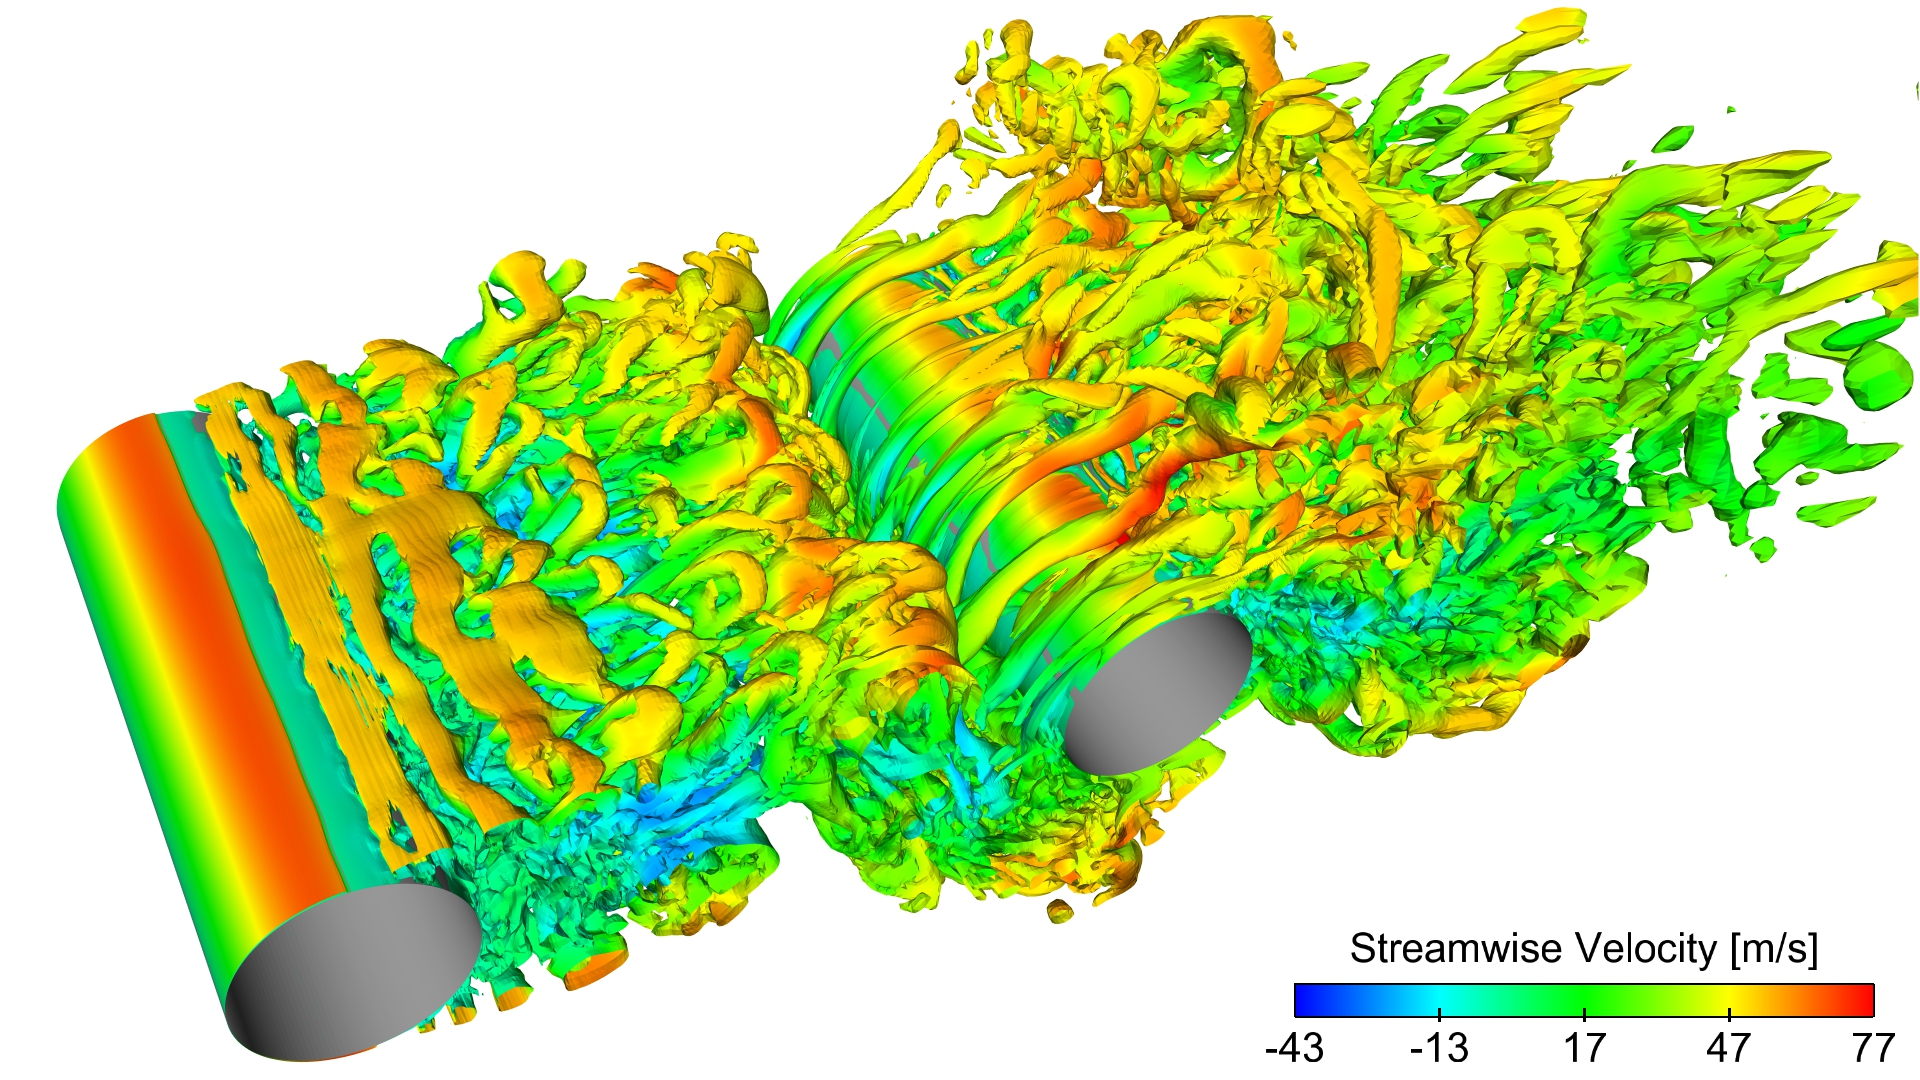
\includegraphics[width=0.45\textwidth]{tc_q_criteria}
    \caption{Q判据等值面图}
    \label{fig:tc_q_criteria}
\end{figure}
\end{verbatim}
\begin{figure}[!htbp]
    \centering
    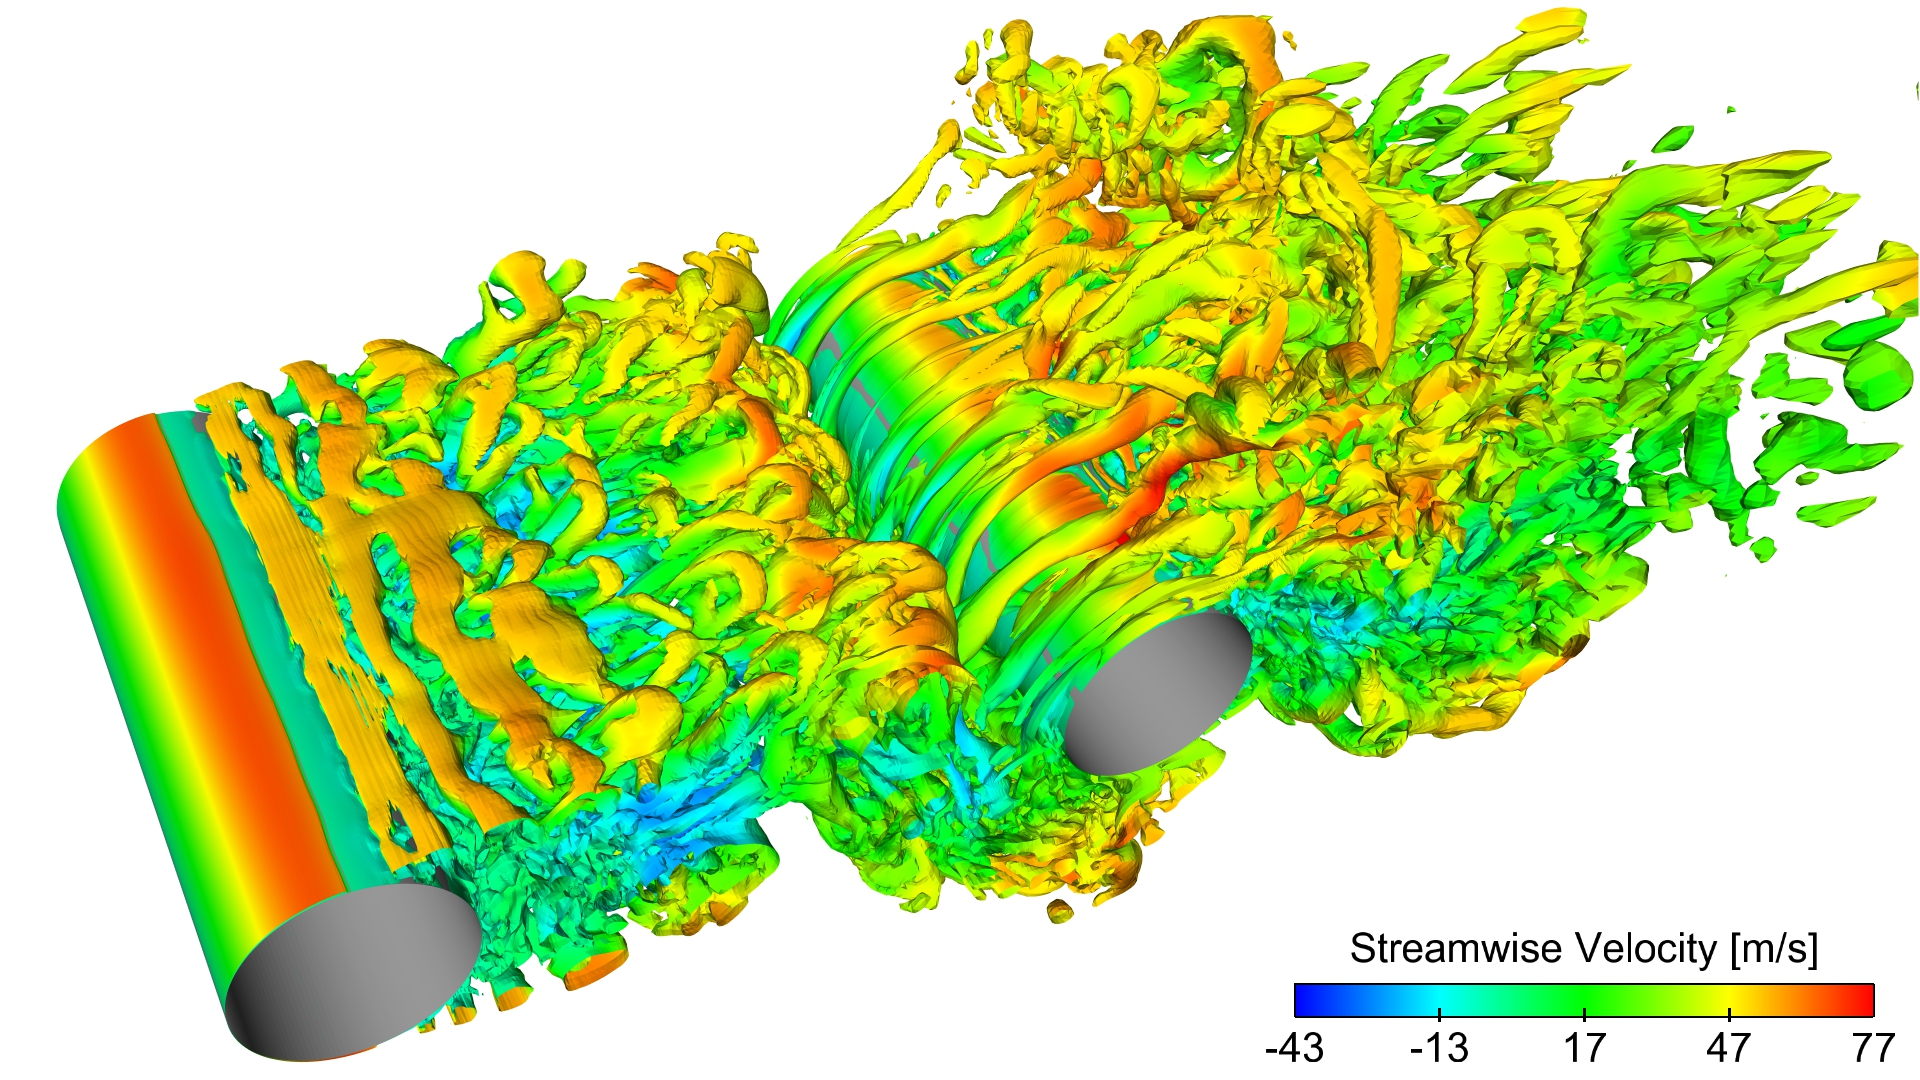
\includegraphics[width=0.45\textwidth]{tc_q_criteria}
    \caption{Q判据等值面图}
    \label{fig:tc_q_criteria}
\end{figure}

如果插图的空白区域过大,希望减少插入图片后的留白,以图片\verb|shock_cyn|为例(图\ref{fig:shock_cyn}),可以使用如下代码模板:
\begin{verbatim}
\begin{figure}[!htbp]
    \centering
    %trim option's parameter order: left bottom right top
    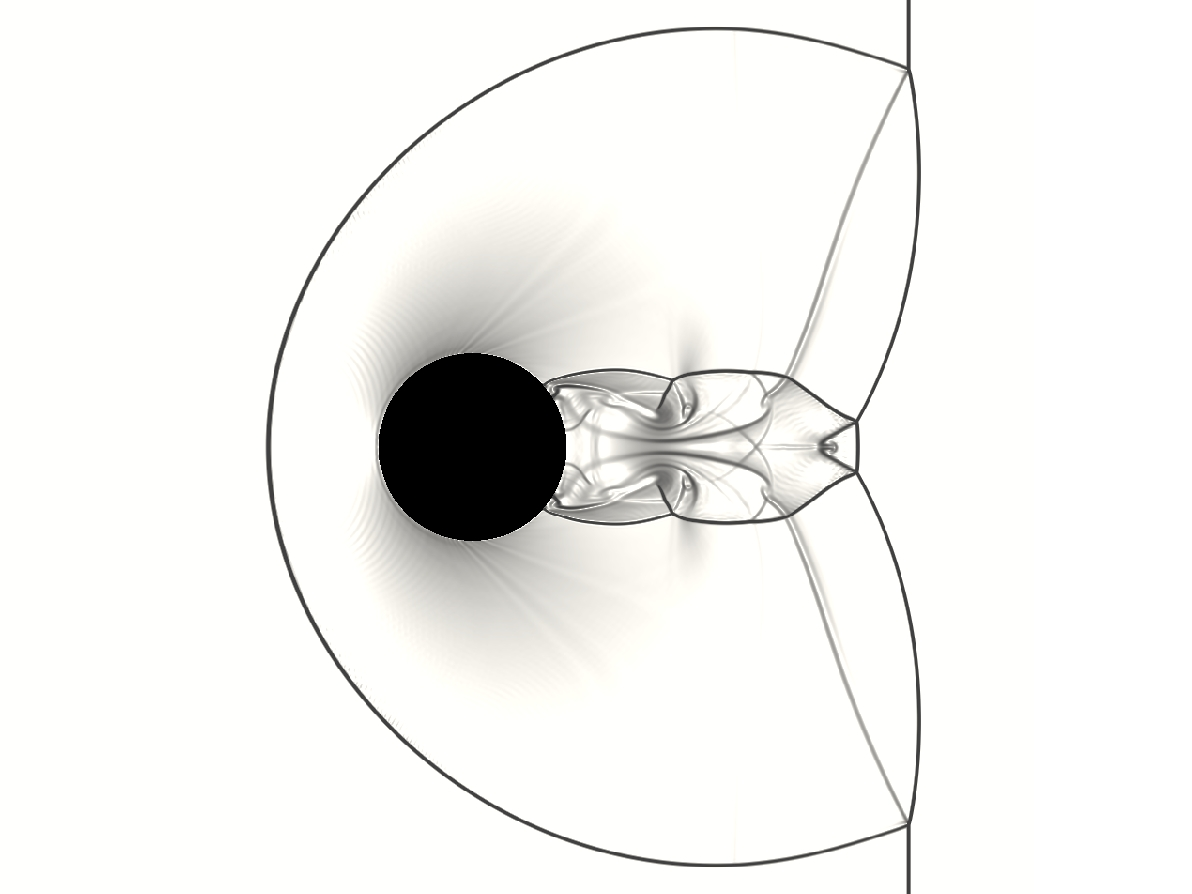
\includegraphics[trim = 30mm 0mm 30mm 0mm, clip,
    width=0.40\textwidth]{shock_cyn}
    \caption{Shock diffraction}
    \label{fig:shock_cyn}
\end{figure}
\end{verbatim}
\begin{figure}[!htbp]
    \centering
    %trim option's parameter order: left bottom right top
    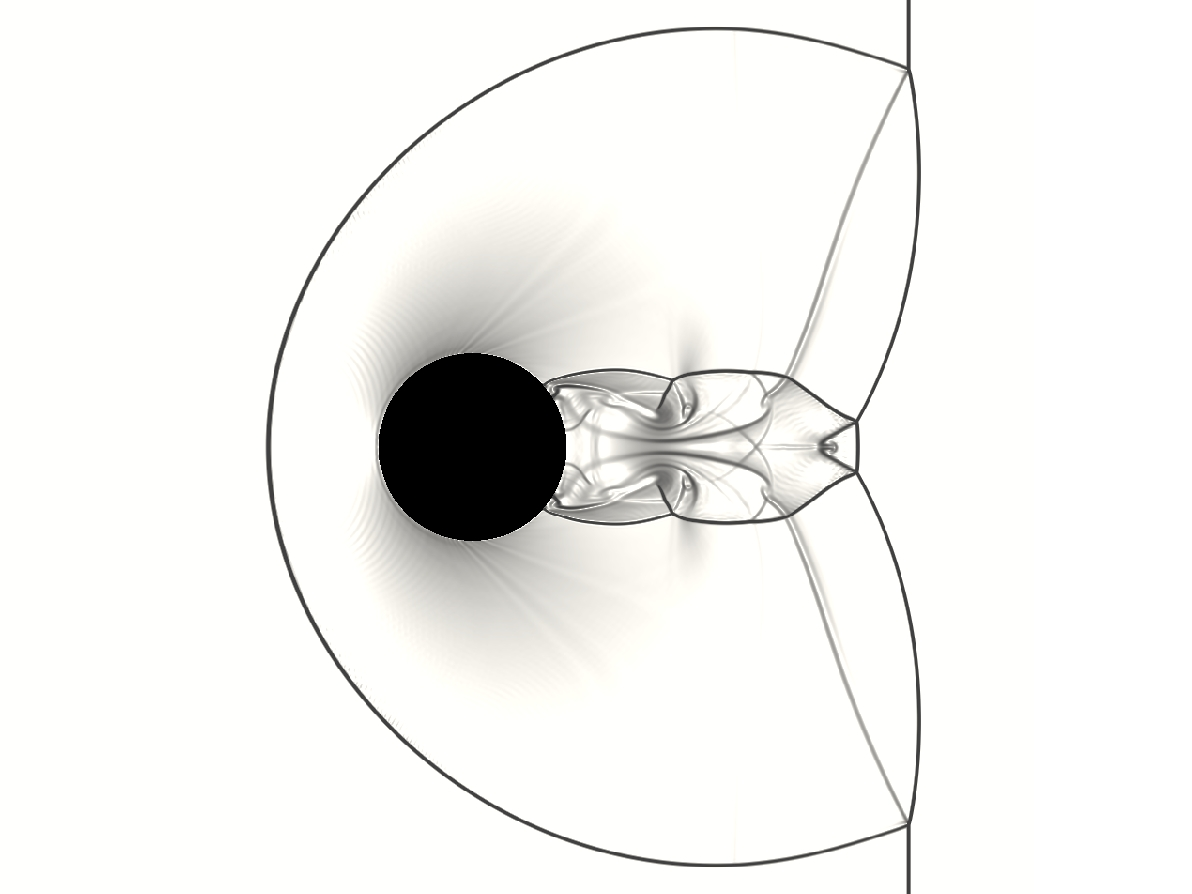
\includegraphics[trim = 30mm 0mm 30mm 0mm, clip, width=0.40\textwidth]{shock_cyn}
    \caption{激波圆柱作用。}
    \label{fig:shock_cyn}
\end{figure}

多图的插入如图\ref{fig:oaspl},其代码如下。
\begin{verbatim}
\begin{figure}[!htbp]
    \centering
    \begin{subfigure}[b]{0.45\textwidth}
      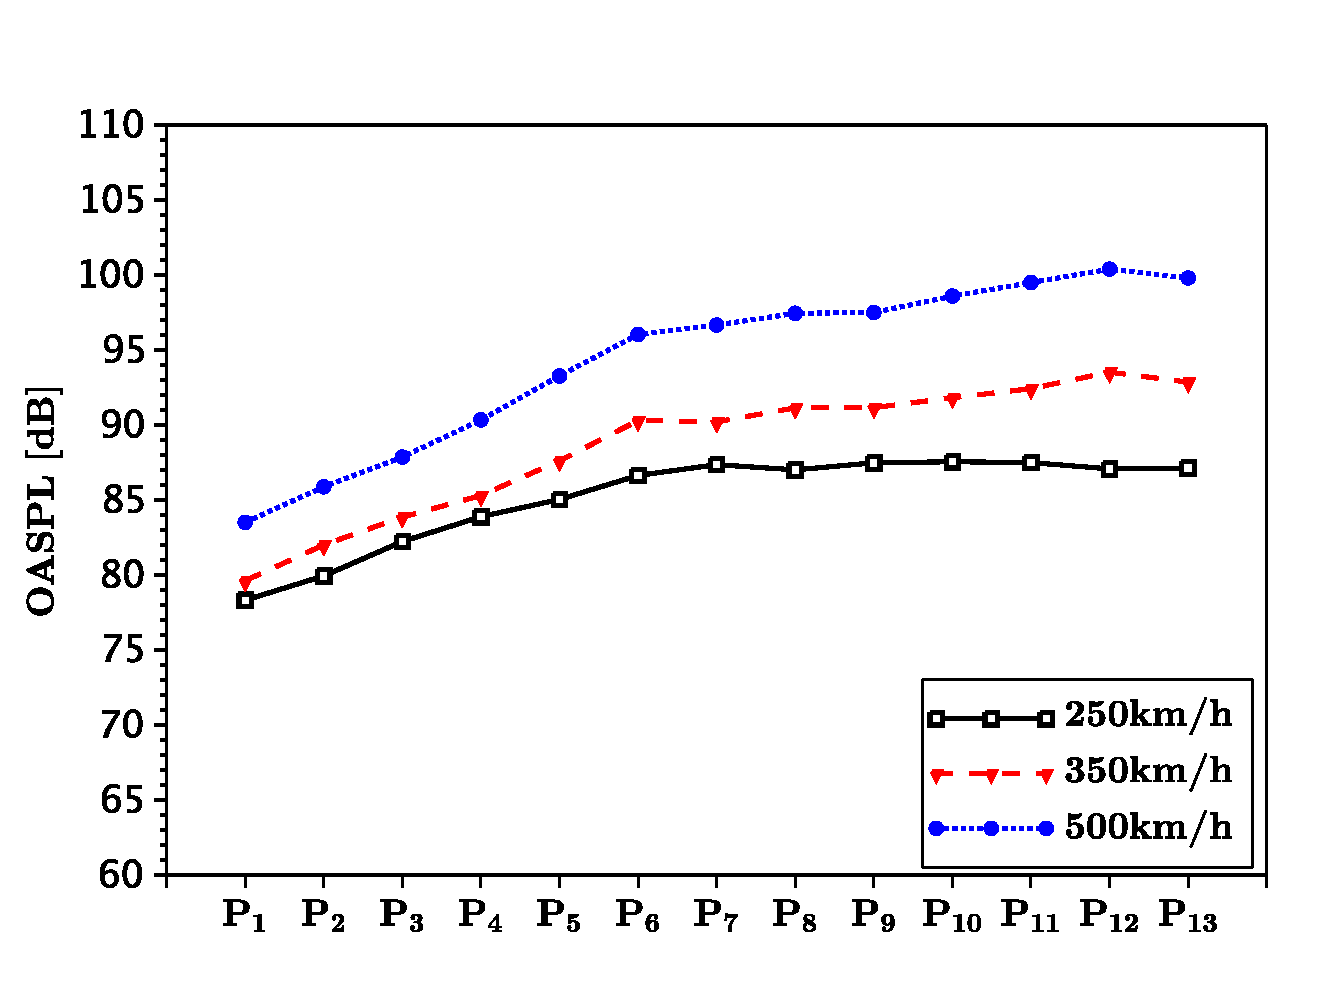
\includegraphics[width=\textwidth]{oaspl_a}
      \caption{}
      \label{fig:oaspl_a}
    \end{subfigure}%
    ~%add desired spacing
    \begin{subfigure}[b]{0.45\textwidth}
      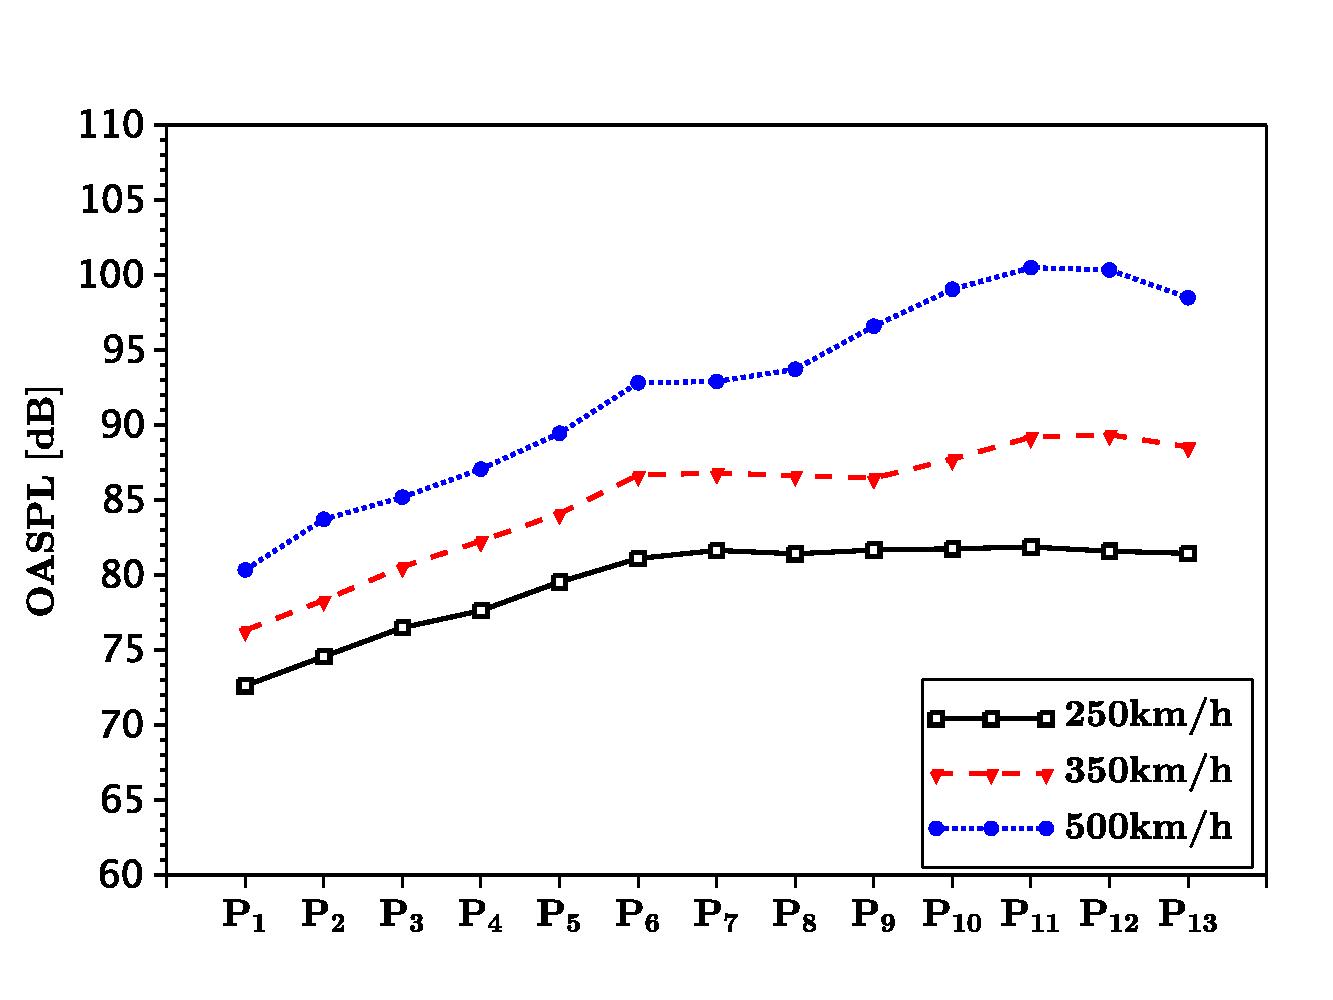
\includegraphics[width=\textwidth]{oaspl_b}
      \caption{}
      \label{fig:oaspl_b}
    \end{subfigure}
    \begin{subfigure}[b]{0.45\textwidth}
      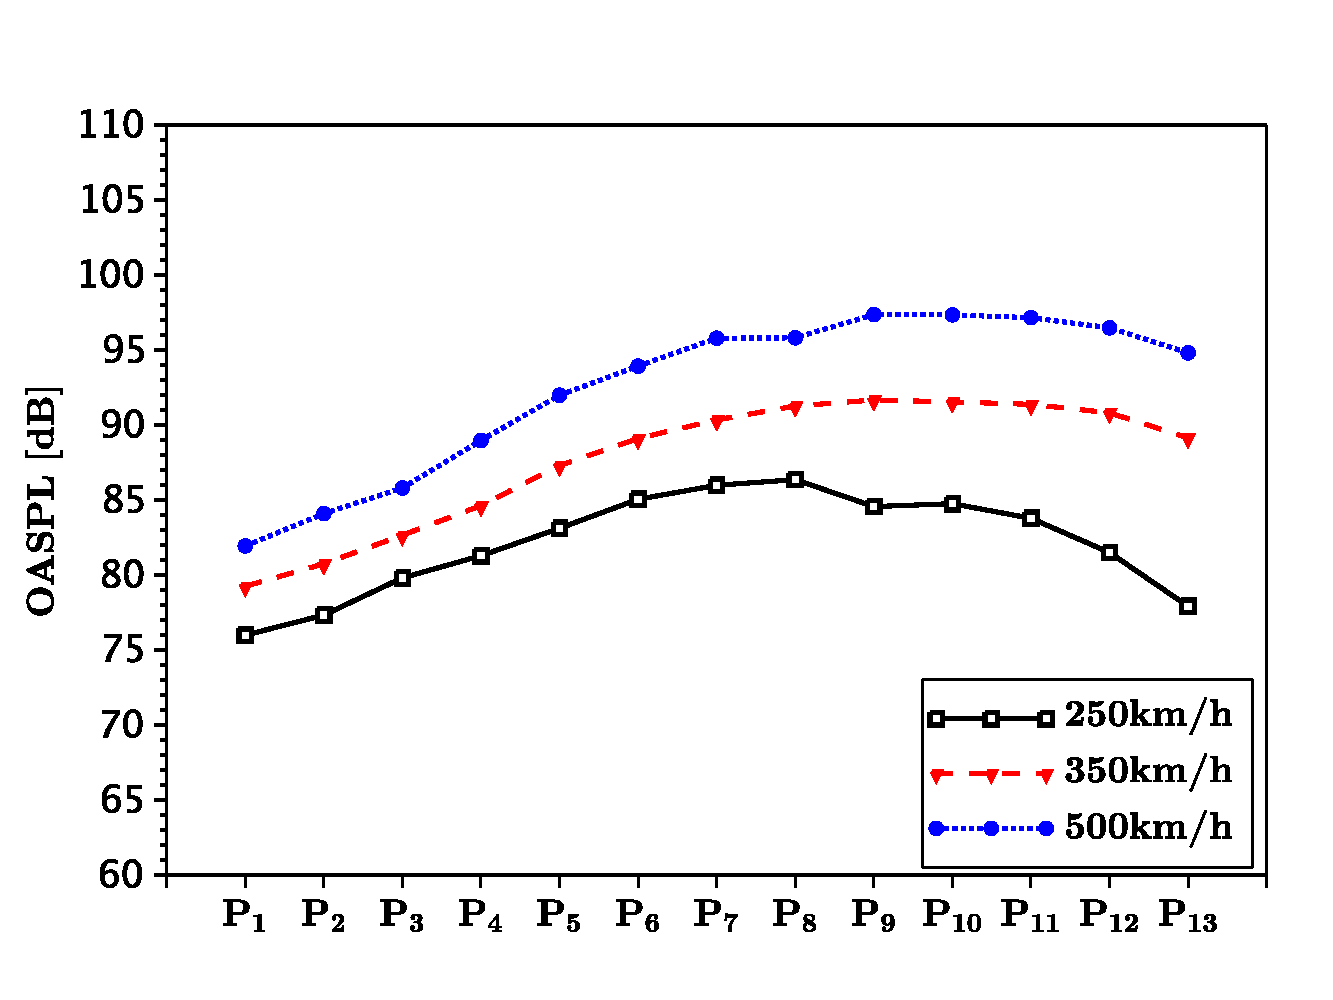
\includegraphics[width=\textwidth]{oaspl_c}
      \caption{}
      \label{fig:oaspl_c}
    \end{subfigure}%
    ~%add desired spacing
    \begin{subfigure}[b]{0.45\textwidth}
      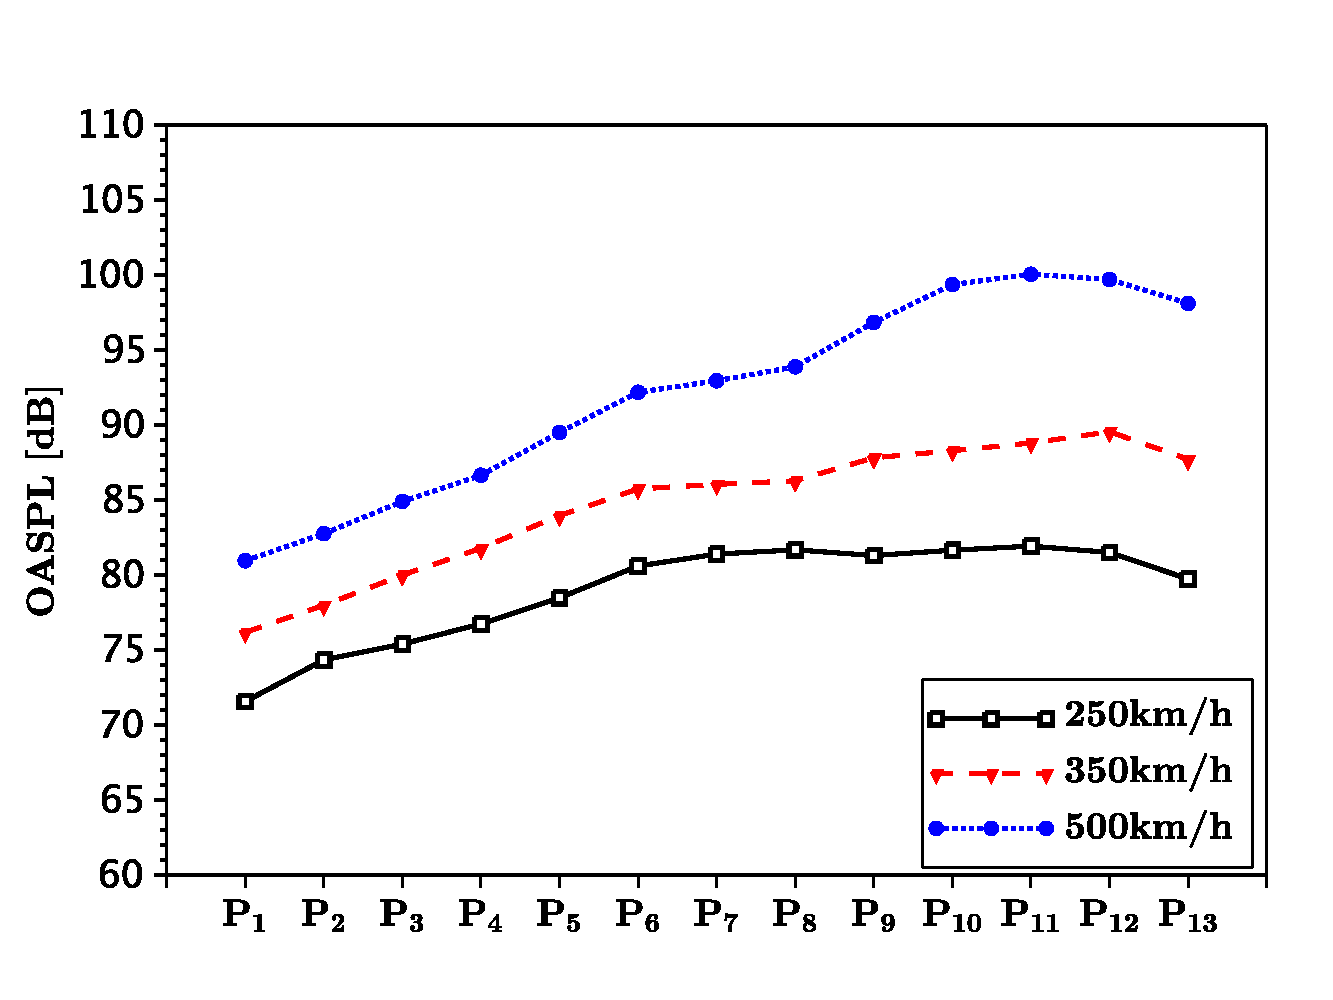
\includegraphics[width=\textwidth]{oaspl_d}
      \caption{}
      \label{fig:oaspl_d}
    \end{subfigure}
    \caption{总声压级。(a)$A$,(b)$B$,(c)$C$,(d)$D$}
    \label{fig:oaspl}
\end{figure}
\end{verbatim}
\begin{figure}[!htbp]
    \centering
    \begin{subfigure}[b]{0.45\textwidth}
      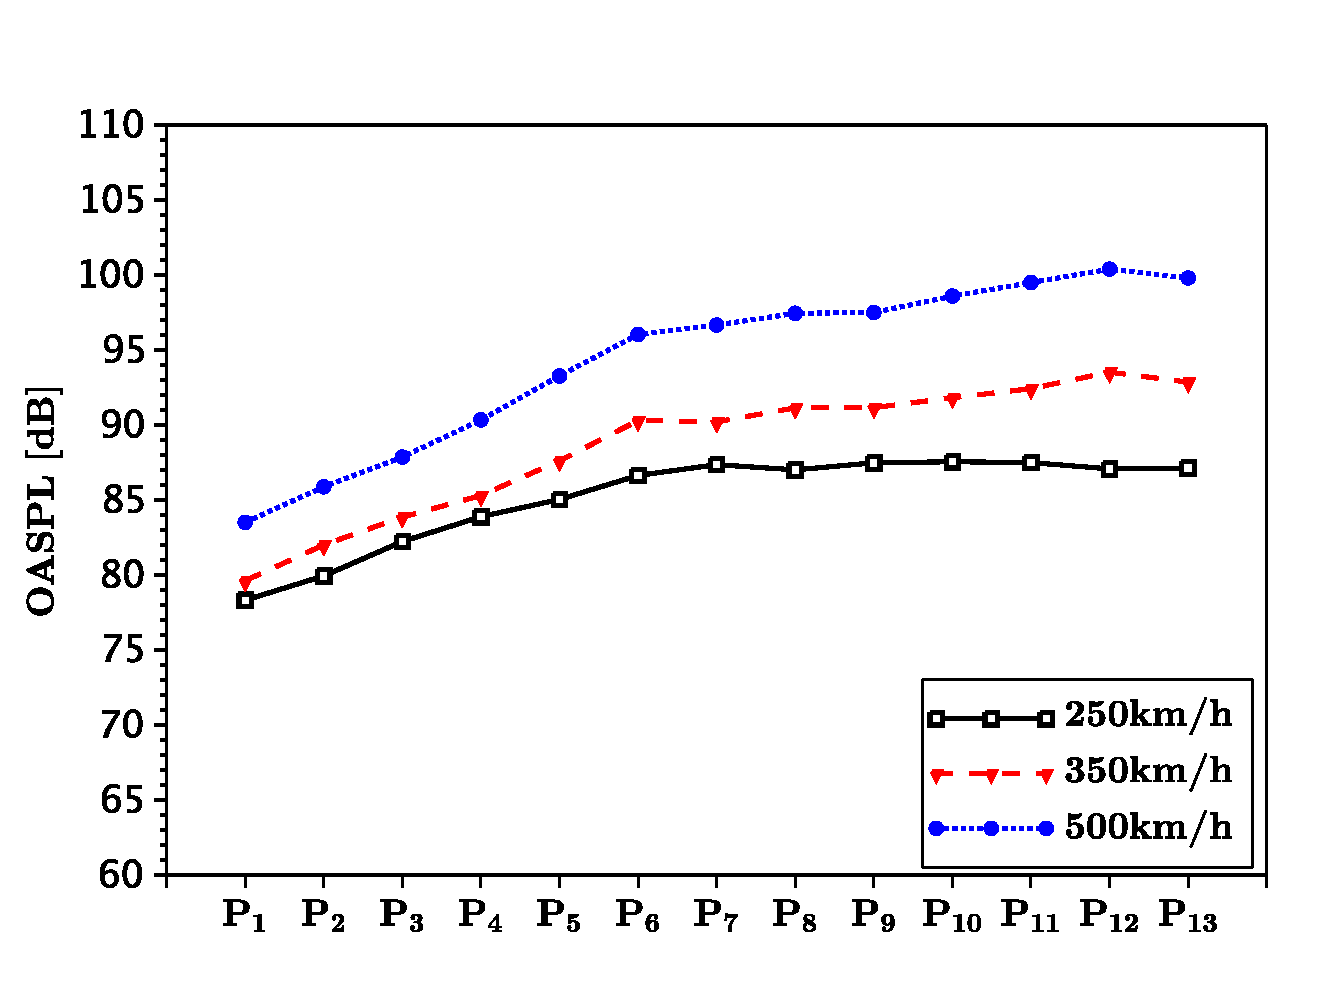
\includegraphics[width=\textwidth]{oaspl_a}
      \caption{}
      \label{fig:oaspl_a}
    \end{subfigure}%
    ~%add desired spacing
    \begin{subfigure}[b]{0.45\textwidth}
      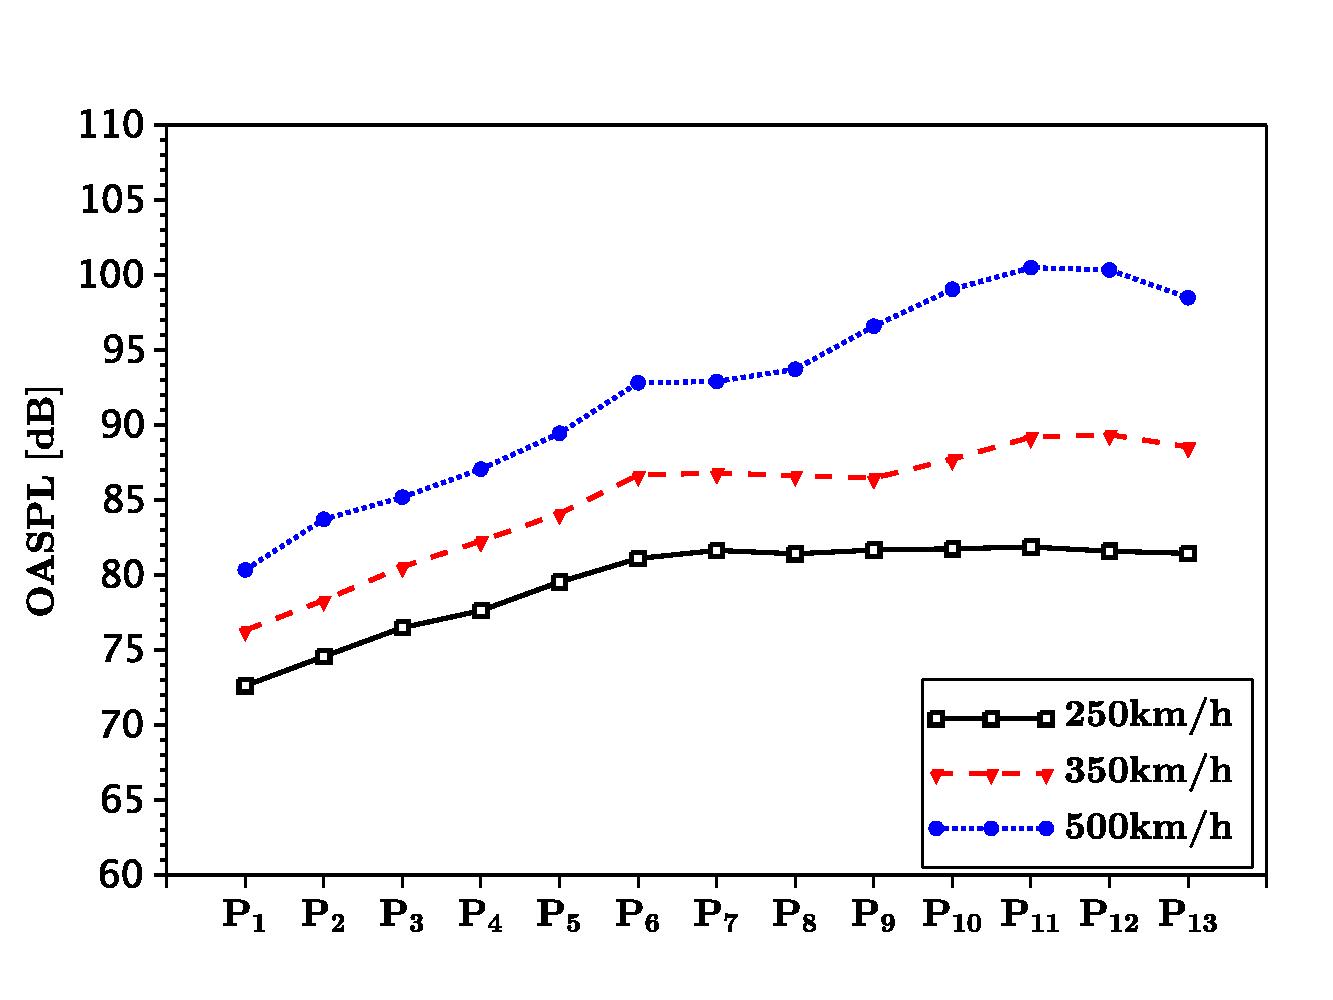
\includegraphics[width=\textwidth]{oaspl_b}
      \caption{}
      \label{fig:oaspl_b}
    \end{subfigure}
    \begin{subfigure}[b]{0.45\textwidth}
      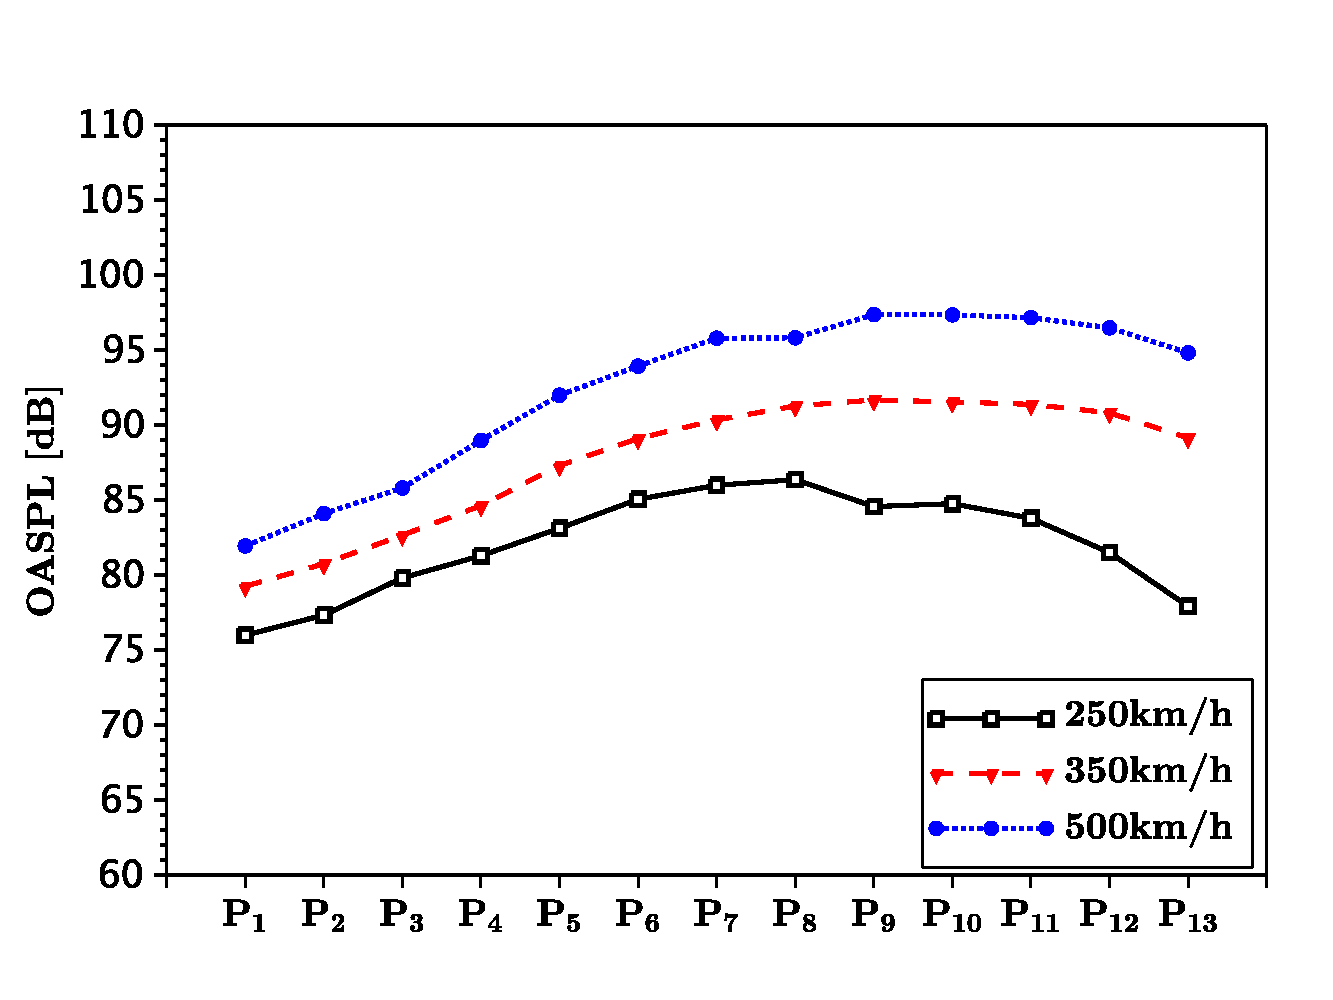
\includegraphics[width=\textwidth]{oaspl_c}
      \caption{}
      \label{fig:oaspl_c}
    \end{subfigure}%
    ~%add desired spacing
    \begin{subfigure}[b]{0.45\textwidth}
      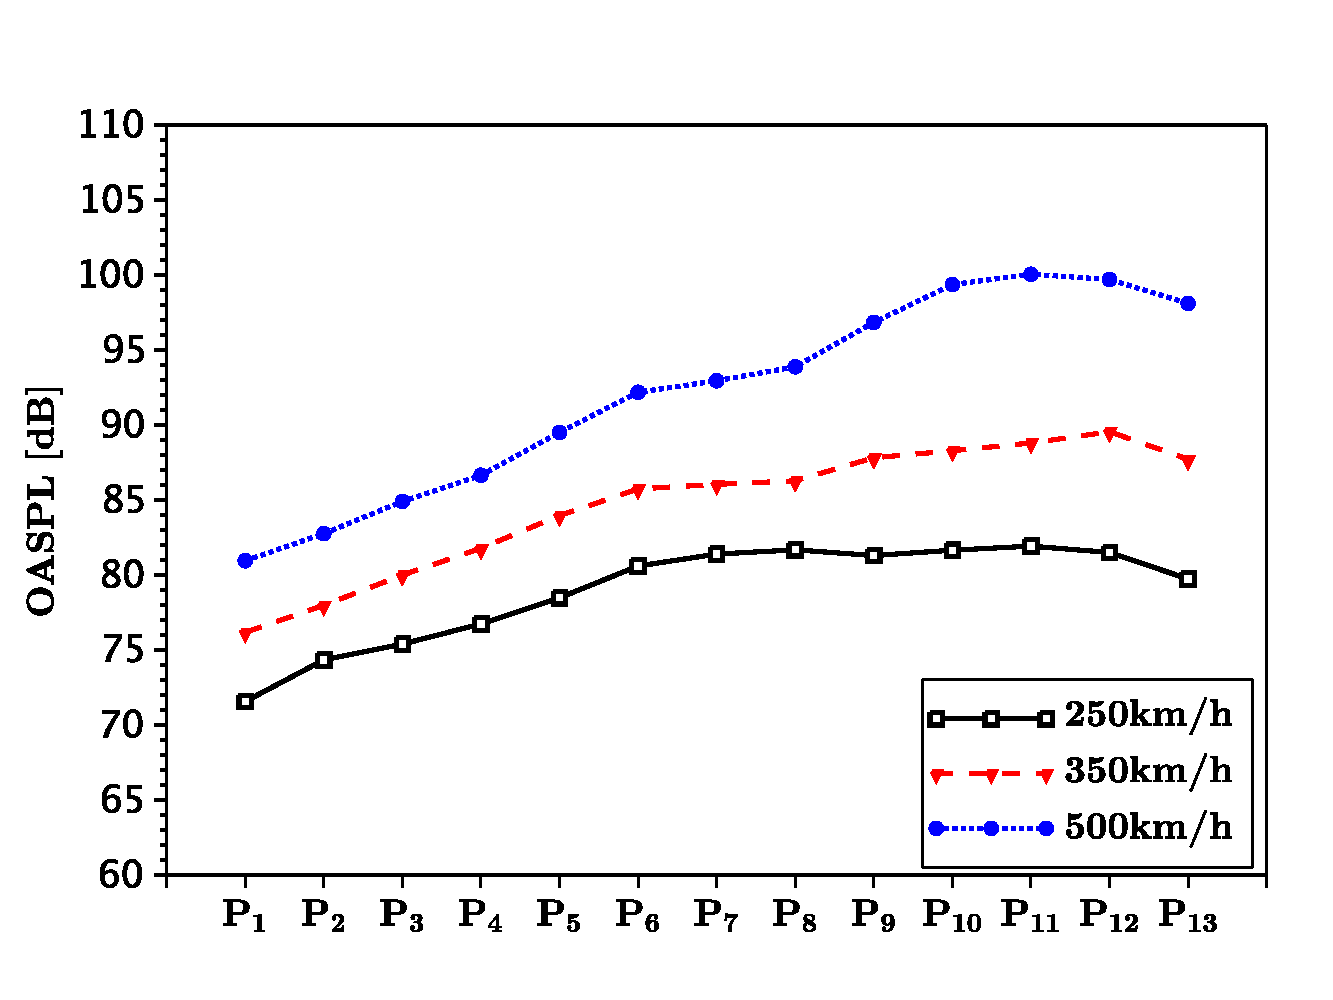
\includegraphics[width=\textwidth]{oaspl_d}
      \caption{}
      \label{fig:oaspl_d}
    \end{subfigure}
    \caption{总声压级。(a)$A$,(b)$B$,(c)$C$,(d)$D$}
    \label{fig:oaspl}
\end{figure}

撰写论文中,插图和制表常用到的命令,已在\verb|Tex/commands.tex|这个文本中给出了参考代码,大家只需拷贝使用即可。

\subsection{参考文献引用}

参考文献引用过程以实例进行介绍,假设需要引用名为"Document Preparation System"的文献,步骤如下:

1)使用Google Scholar搜索Document Preparation System,在目标条目下点击Cite,展开后选择Import into BibTeX打开此文章的BibTeX索引信息,将它们copy添加到ref.bib文件中(此文件位于Biblio文件夹下)。

2)你会发现索引信息中第一行为 \verb|@article{lamport1986document,|。其中 \verb|lamport1986document| 即为此文献的label (\textbf{中文文献也必须使用英文label},一般遵照:姓氏拼音+年份+标题第一字拼音的格式),想要在论文中索引此文献,有两种索引类型:

文本类型:\verb|\citet{lamport1986document}|。正如此处所示 \citet{lamport1986document}; 

括号类型:\verb|\citep{lamport1986document}|。正如此处所示 \citep{lamport1986document}。

\textbf{多文献索引用英文逗号隔开}:

\verb|\citep{lamport1986document,chen2005zhulu}|。正如此处所示 \citep{lamport1986document,chen2005zhulu}

如此,即完成了文献的索引,请查看下本文档的参考文献一章,看看是不是就是这么简单呢?是的,就是这么简单!

不同文献样式和引用样式可在Thesis.tex中对artratex.sty调用实现,如:
\begin{itemize}
    \item \verb+\usepackage[numbers]{artratex}+ $\%$ textual: Jones [1]; parenthetical: [1]
    \item \verb+\usepackage[super]{artratex}+ $\%$ textual: Jones 上标[1]; parenthetical: 上标[1]
    \item \verb+\usepackage[authoryear]{artratex}+ $\%$ textual: Jones (1995); parenthetical: (Jones, 1995)
    \item \verb+\usepackage[alpha]{artratex}+ $\%$ textual: not available; parenthetical: [Jon95]
\end{itemize}

若在上标(super)模式下,希望在特定位置将上标改为嵌入式标,可使用

文本类型:\verb|\citetns{lamport1986document,chen2005zhulu}|。正如此处所示\citetns{lamport1986document,chen2005zhulu}

括号类型:\verb|\citepns{lamport1986document,chen2005zhulu}|。正如此处所示\citepns{lamport1986document,chen2005zhulu}

参考文献索引更为详细的信息,请见Wikibook\citep{wikibook2014latex} \nocite{*}。

\section{常见使用问题}\label{sec:qa}

\begin{enumerate}
    \item 下载模板后,用脚本编译出现错误,则i)请下载并更新模板。请更新\LaTeX{}编译器和包裹库,以确保模板与编译器的匹配。ii) 编译中若出现缺乏包裹或字体并提示是否自动下载,请选择自动下载,即可解决大部分初始编译时所遇到的问题。本模板在每次修改的发布前,都已在Windows,Linux,Mac OS系统的最近两个发行版的Texlive上测试通过。

    \item 模板文档的编码为UTF-8编码。所有文件都必须采用UTF-8编码,否则编译后生成的文档将出现乱码文本。若出现文本编辑器无法打开文档或打开文档乱码的问题,请检查您使用的编辑器对UTF-8编码的支持。如果使用WinEdt作为文本编辑器(不推荐使用),应在其Options -> Preferences -> wrapping选项卡下将两种Wrapping Modes中的内容:TeX;HTML;ANSI;ASCII|DTX...修改为:TeX;\textbf{UTF-8|ACP;}HTML;ANSI;ASCII|DTX...同时,取消Options -> Preferences -> Unicode中的Enable ANSI Format...选项。

    \item 推荐选择xelatex编译引擎编译中文文档。编译脚本的默认设定为xelatex编译引擎。你也可以选择不使用脚本编译,如直接使用 \TeX{}文本编辑器编译。注:\TeX{}文本编辑器编译的默认设定为pdflatex编译引擎,若选择xelatex编译引擎,请进入下拉菜单选择xelatex。为正确生成引用链接,需要进行全编译,其步骤为:\verb|xelatex + bibtex + xelatex + xelatex|。
    \item Texmaker使用简介
        \begin{enumerate}
            \item 使用 Texmaker 打开文档 Thesis.tex。
            \item 菜单 Options -> Define Current Document As 'Master Document'
            \item 菜单 User -> User Commands -> Edit User Commands -> Input Menu Item as 'Auto Build' -> Click 'wizard' -> add: xelatex + bibtex + xelatex + xelatex + pdf viewer -> Click 'OK'
            \item 使用 Auto Build 编译带有未生成引用链接的源文件,可以仅使用 xelatex 编译带有已经正确生成引用链接的源文件。
            \item 编译完成,View PDF,在pdf中'ctrl+click'可链接到相对应的源文件。
        \end{enumerate}

    \item 若编译过程中出现无法找到某些package的错误,如无法找到xcolor.sty,mathtools.sty,ctexbook.sty,newtext.sty等,\TeX{}编译程序一般可以自动下载和安装相应的文件,否则,请进入\LaTeX{}软件的Package Manager (Admin)确认启用Repository--Synchronize状态。下次编译过程中\TeX{}编译程序一般将自动下载安装\LaTeX{}宏包库。
    \item 模版的设计可能地考虑了适应性。致谢等所有条目都是通过最为通用的

        \verb+\chapter{item name}+  and \verb+\section*{item name}+

        来显式实现的 (请观察Backmatter.tex),从而可以随意添加,放置,和修改,如同一般章节。对于图表目录名称则可在ucasthesis.cfg中进行修改。

    \item 设置文档样式: 在artratex.sty中搜索关键字定位相应命令,然后修改
        \begin{enumerate}
            \item 正文行距:修改 \verb|\linespread{1.3}|
            \item 参考文献行距:修改\verb|\setlength{\bibsep}{0.0ex}|
            \item 目录显示subsection:修改\verb|\setcounter{tocdepth}{2}|
            \item 页眉页脚的设定:frontmatterstyle,mainmatterstyle,和backmatterstyle分别用于定义前言,主要内容,和附录的页眉页脚样式。                关于页眉页脚各个命令的作用和意义请参见fancyhdr的用户文档 \url{https://www.ctan.org/pkg/fancyhdr?lang=en}。同时参见ctex宏包用户文档
                
                \url{http://ctan.mirror.rafal.ca/language/chinese/ctex/ctex.pdf}

            \item 设置图2.3为图2-3: 设置
\begin{verbatim}
  \renewcommand{\theequation}{\arabic{chapter}-\arabic{equation}}
  \renewcommand{\thefigure}{\arabic{chapter}-\arabic{figure}}
  \renewcommand{\thetable}{\arabic{chapter}-\arabic{table}}
\end{verbatim}
             \item 字体控制。如果对字体控制有较高需求,请选择xelatex编译引擎,并设置需要的字体,如启用Times New Roman 作为英文字体,设置:

                 \verb+\setmainfont{Times New Roman}+
        \end{enumerate}

    \item 在某些情况下拷贝pdf文档内容到word时存在乱码。解决方式是选择安装adobe相应的字体库,请在公共网站(如百度云盘:\url{http://pan.baidu.com/share/home?uk=3188136325&view=share#category/type=0})搜索并下载如下四种中文字体文件:
        \begin{enumerate}
            \item AdobeFangsongStd-Regular.otf (adobe 仿宋)
            \item AdobeHeitiStd-Regular.otf(adobe 黑体)
            \item AdobeKaitiStd-Regular.otf(adobe 楷体)
            \item AdobeSongStd-Light.otf(adobe 宋体)
        \end{enumerate}
        下载后,双击安装相应字体。然后在Thesis.tex中设置启用adobe的字体:

      \verb+\documentclass[doublesided,fontset=adobe]{Style/ucasthesis}%+

     最后选择xelatex编译引擎编译。因为模版的设定考虑兼顾不同操作系统(Windows, Linux, Mac OS)并兼顾pdflatex和xelatex,为了模版的健壮性,上述方案并未作为原始设定。

 \item  一般规范下,章应开始于奇数页。从而若前一章结束于奇数页,则一空白页将被插入以保证上述规则。如想修改以取消空白页,有如下方案:
     \begin{itemize}
         \item 在thesis.tex的documentclass中用singlesided替代doublesided。这使文档不区分奇偶页,因此章可以开始于任意页。此方案将移除所有空白页,包括封面处的。同时,页眉页脚的设定不再区分奇偶页。
         \item 可以在ucasthesis.cls文件中,将cleardoublepage命令的定义修改为:

             \verb|\def\cleardoublepage{\clearpage}|

             这一命令使产生空白页的机制失效。这一方案将移除所有的空白页,包括封面处的。但与方案一不同的是,页面页脚的设定可以区分奇偶页。
         \item 在thesis.tex的documentclass中添加openany选项(openany与doublesided和printcopy都可搭配)。这一命令使章可以开始于任意页。同时,将artratex.sty中和thesis.tex中的cleardoublepage改为clearpage。此方案将移除所有的用于调整章的起始位置的空白页,而不包括封面处的。同时,页面页脚的设定可以区分奇偶页。
     \end{itemize}
      无论哪种方案都要注意对页眉页脚的影响并做出合适的调整。推荐是采用默认设置,尽量避免将精力花在这些无关紧要的细节上。\LaTeX{}的特点是标准化,而其导致的问题则是任何脱离标准的修改都将花费相当精力。对于电子档的论文,在thesis.tex的documentclass中,若不想使用doublesided,则可使用singlesided来减少空白页。而对于打印版,启用printcopy选项以替换doublesided/singlesided选项,这样可使奇偶页的排版在打印装订后更美观。
  \item 部分所也许对论文格式有不同的设定,\LaTeX{}用户亦无需担心,仍可放心地使用当前模板进行论文撰写,因为\LaTeX{}的特征就在于内容与格式的分离。在使用此模板完成论文的撰写后,任何形式的格式调整都可独立于内容进行,并可只需通过修改模板样式文件中的少数命令轻松快速完成,并无风险。
\end{enumerate}




%---------------------------------------------------------------------------%
% main content
%-
%-> Appendix
%-
% \cleardoublepage%
% \appendix% initialize the environment
% 
\chapter{中国科学院大学学位论文撰写要求}

学位论文是研究生科研工作成果的集中体现,是评判学位申请者学术水平、授予其学位的主要依据,是科研领域重要的文献资料。根据《科学技术报告、学位论文和学术论文的编写格式》(GB/T 7713-1987)、《学位论文编写规则》(GB/T 7713.1-2006)和《文后参考文献著录规则》(GB7714—87)等国家有关标准,结合中国科学院大学(以下简称“国科大”)的实际情况,特制订本规定:\url{http://onestop.ucas.edu.cn/home/info/abc167cb-4589-4e05-b014-052fa9291d0c/1}。
% appendix content
%-
%-> Backmatter: bibliography, glossary, index
%-
% \backmatter% initialize the environment
% \intotoc{\bibname}% add link to contents table and bookmark
% \bibliography{Biblio/ref}% bibliography
% \chapter{作者简历及攻读学位期间发表的学术论文与研究成果}

\section*{作者简历}

\subsection*{casthesis作者}

吴凌云,男,福建省屏南县人,1975 年出生,中国科学院数学与系统科学研究院博士研究生。

通讯地址:北京市~2734 信箱,中科院数学与系统科学研究院应用数学所

邮编:100080

E-mail: aloft@ctex.org

\subsection*{ucasthesis作者}

莫晃锐,男,湖南省湘潭县人,1989 年出生,中国科学院力学研究所硕士研究生。

通讯地址:北京市北四环西路15号中国科学院力学研究所

邮编:100190

E-mail: mohuangrui@gmail.com

\section*{已发表(或正式接受)的学术论文:}

[1] Thesis Template of the University of Chinese Academy of Sciences, 2014.

\section*{申请或已获得的专利:}

(无专利时此项不必列出)

\section*{参加的研究项目及获奖情况:}

可以随意添加新的条目或是结构

\chapter{致\quad 谢}

值此论文完成之际,谨在此向多年来给予我关心和帮助的老师、学长、同学、
朋友和家人表示衷心的感谢!

没有~ctex package~的众多前辈的辛勤付出和~CASthesis package~作者吴凌云学长的贡献,
~\LaTeX{}~菜鸟的我是无法完成此学位论文模板的。在~\LaTeX{}~中的一点一滴的成长源于
开源社区的众多资料和教程,在此对所有前辈们的付出表示感谢!

......

谨把本文献给我最敬爱的父亲!
% other information
\end{document}
%---------------------------------------------------------------------------%
